\documentclass[11pt,compress,t,notes=noshow, xcolor=table, aspectratio=169]{beamer}
\usepackage[]{graphicx}

\usepackage[]{color}
% maxwidth is the original width if it is less than linewidth
% otherwise use linewidth (to make sure the graphics do not exceed the margin)
\makeatletter
\def\maxwidth{ %
  \ifdim\Gin@nat@width>\linewidth
    \linewidth
  \else
    \Gin@nat@width
  \fi
}
\makeatother

\definecolor{fgcolor}{rgb}{0.345, 0.345, 0.345}
\newcommand{\hlnum}[1]{\textcolor[rgb]{0.686,0.059,0.569}{#1}}%
\newcommand{\hlstr}[1]{\textcolor[rgb]{0.192,0.494,0.8}{#1}}%
\newcommand{\hlcom}[1]{\textcolor[rgb]{0.678,0.584,0.686}{\textit{#1}}}%
\newcommand{\hlopt}[1]{\textcolor[rgb]{0,0,0}{#1}}%
\newcommand{\hlstd}[1]{\textcolor[rgb]{0.345,0.345,0.345}{#1}}%
\newcommand{\hlkwa}[1]{\textcolor[rgb]{0.161,0.373,0.58}{\textbf{#1}}}%
\newcommand{\hlkwb}[1]{\textcolor[rgb]{0.69,0.353,0.396}{#1}}%
\newcommand{\hlkwc}[1]{\textcolor[rgb]{0.333,0.667,0.333}{#1}}%
\newcommand{\hlkwd}[1]{\textcolor[rgb]{0.737,0.353,0.396}{\textbf{#1}}}%
\let\hlipl\hlkwb

\usepackage{framed}
\makeatletter
\newenvironment{kframe}{%
 \def\at@end@of@kframe{}%
 \ifinner\ifhmode%
  \def\at@end@of@kframe{\end{minipage}}%
  \begin{minipage}{\columnwidth}%
 \fi\fi%
 \def\FrameCommand##1{\hskip\@totalleftmargin \hskip-\fboxsep
 \colorbox{shadecolor}{##1}\hskip-\fboxsep
     % There is no \\@totalrightmargin, so:
     \hskip-\linewidth \hskip-\@totalleftmargin \hskip\columnwidth}%
 \MakeFramed {\advance\hsize-\width
   \@totalleftmargin\z@ \linewidth\hsize
   \@setminipage}}%
 {\par\unskip\endMakeFramed%
 \at@end@of@kframe}
\makeatother

\definecolor{shadecolor}{rgb}{.97, .97, .97}
\definecolor{messagecolor}{rgb}{0, 0, 0}
\definecolor{warningcolor}{rgb}{1, 0, 1}
\definecolor{errorcolor}{rgb}{1, 0, 0}
\newenvironment{knitrout}{}{} % an empty environment to be redefined in TeX

\newcommand{\SweaveOpts}[1]{}  % do not interfere with LaTeX
\newcommand{\SweaveInput}[1]{} % because they are not real TeX commands
\newcommand{\Sexpr}[1]{}       % will only be parsed by R
\newcommand{\xmark}{\ding{55}}%

\usepackage{alltt}
\usepackage[utf8]{inputenc}

\usepackage[english]{babel}
\usepackage{dsfont}
\usepackage{verbatim}
\usepackage{amsmath}
\usepackage{amsfonts}
\usepackage{amssymb}
\usepackage{bm}
\usepackage{csquotes}
\usepackage{multirow}
\usepackage{longtable}
\usepackage{booktabs}
\usepackage{enumerate}
\usepackage[absolute,overlay]{textpos}
\usepackage{psfrag}
\usepackage{algorithm}
\usepackage{algpseudocode}
\usepackage{eqnarray}
\usepackage{arydshln}
\usepackage{tabularx}
\usepackage{placeins}
\usepackage{tikz}
\usepackage{setspace}
\usepackage{colortbl}
\usepackage{mathtools}
\usepackage{wrapfig}
\usepackage{bm}
\usepackage{amsmath}
\usepackage{pifont}
\usepackage{xcolor} %colored math symbols
\usepackage{adjustbox}
\usepackage{verbatimbox}
\usepackage{tcolorbox}
\usepackage{siunitx}
\def\signed #1{{\leavevmode\unskip\nobreak\hfil\penalty50\hskip1em
  \hbox{}\nobreak\hfill #1%
  \parfillskip=0pt \finalhyphendemerits=0 \endgraf}}

% basic latex stuff
\newcommand{\col}{\par\colorbox{code}{\parbox{\textwidth}{\theverbbox}}\par}


\usetikzlibrary{shapes,arrows,automata,positioning,calc,chains,trees, shadows}
\tikzset{
  %Define standard arrow tip
  >=stealth',
  %Define style for boxes
  punkt/.style={
    rectangle,
    rounded corners,
    draw=black, very thick,
    text width=6.5em,
    minimum height=2em,
    text centered},
  % Define arrow style
  pil/.style={
    ->,
    thick,
    shorten <=2pt,
    shorten >=2pt,}
}

\newsavebox\mybox
\newenvironment{aquote}[1]
  {\savebox\mybox{#1}\begin{quote}\openautoquote\hspace*{-.7ex}}
  {\unskip\closeautoquote\vspace*{1mm}\signed{\usebox\mybox}\end{quote}}

\usepackage{subfig}

% Defines macros and environments
\usepackage{../style/dhbw-lecture}


\let\code=\texttt
\let\proglang=\textsf

\setkeys{Gin}{width=0.9\textwidth}

% The accent rule sits on its own vbox line with \nointerlineskip so it costs
% only its own 1.2pt height + the explicit 2pt gap, instead of pulling in a
% full \baselineskip (~0.6-0.7cm) the way a plain "\\" line break would --
% that overhead on every single frame is what was pushing picture-heavy
% frames over the shorter 16:9 frame height.
\setbeamertemplate{frametitle}{\expandafter\uppercase\expandafter\insertframetitle\par\vskip2pt\nointerlineskip\hbox{\color{dhbwaccent}\rule{1.6cm}{1.2pt}}}
\addtobeamertemplate{frametitle}{}{\vspace{0.08cm}}

\usepackage{bbm}
% basic latex stuff
\newcommand{\pkg}[1]{{\fontseries{b}\selectfont #1}} %fontstyle for R packages
\newcommand{\lz}{\vspace{0.5cm}} %vertical space
\newcommand{\dlz}{\vspace{1cm}} %double vertical space
\newcommand{\oneliner}[1] % Oneliner for important statements
{\begin{block}{}\begin{center}\begin{Large}#1\end{Large}\end{center}\end{block}}


%new environments
\newenvironment{vbframe}  %frame with breaks and verbatim
{
 \begin{frame}[containsverbatim,allowframebreaks]
}
{
\end{frame}
}

\newenvironment{vframe}  %frame with verbatim without breaks (to avoid numbering one slided frames)
{
 \begin{frame}[containsverbatim]
}
{
\end{frame}
}

\newenvironment{blocki}[1]   % itemize block
{
 \begin{block}{#1}\begin{itemize}
}
{
\end{itemize}\end{block}
}

\newenvironment{fragileframe}[2]{  %fragile frame with framebreaks
\begin{frame}[allowframebreaks, fragile, environment = fragileframe]
\frametitle{#1}
#2}
{\end{frame}}


\newcommand{\myframe}[2]{  %short for frame with framebreaks
\begin{frame}[allowframebreaks]
\frametitle{#1}
#2
\end{frame}}

\newcommand{\remark}[1]{
  \textbf{Remark:} #1
}


\newenvironment{deleteframe}
{
\begingroup
\usebackgroundtemplate{
\includegraphics[width=\paperwidth,height=\paperheight]{../style/color/red.png}}
 \begin{frame}
}
{
\end{frame}
\endgroup
}
\newenvironment{simplifyframe}
{
\begingroup
\usebackgroundtemplate{
\includegraphics[width=\paperwidth,height=\paperheight]{../style/color/yellow.png}}
 \begin{frame}
}
{
\end{frame}
\endgroup
}\newenvironment{draftframe}
{
\begingroup
\usebackgroundtemplate{
\includegraphics[width=\paperwidth,height=\paperheight]{../style/color/green.jpg}}
 \begin{frame}
}
{
\end{frame}
\endgroup
}
% https://tex.stackexchange.com/a/261480: textcolor that works in mathmode
\makeatletter
\renewcommand*{\@textcolor}[3]{%
  \protect\leavevmode
  \begingroup
    \color#1{#2}#3%
  \endgroup
}
\makeatother


\input{../latex-math/basic-math}
\input{../latex-math/basic-ml}
\input{../latex-math/ml-nn}

\newcommand{\titlefigure}{figure/vae_faces.png}
\newcommand{\learninggoals}{
  \item RNNs as the sequence-processing counterpart to CNNs' spatial processing: parameter sharing across time, and backpropagation through time
  \item LSTM and GRU cells as fixes for the vanishing-gradient problem in vanilla RNNs
  \item RNN application patterns: language modeling, word embeddings, encoder-decoder (seq2seq) architectures
  \item Autoencoders as unsupervised feature learners: the undercomplete bottleneck, the connection to PCA, and regularized variants (sparse, denoising, contractive)
  \item Variational Autoencoders (VAEs) as probabilistic generative models: the ELBO objective and the reparameterization trick, at the concept level
}

\title{Advanced Artificial Intelligence and Machine Learning}
\date{}

\begin{document}

\lecturechapter{Sequential \& Generative Models}
\lecture{Advanced AI \& ML}
%%%%%%%%%%%%%%%%%%%%%%%%%%%%%%%%%%%%%%%%%%%%%%%%%%%%%%%%%%%%%%%%%%

\section{RNN: Motivation and Mechanics}
%%%%%%%%%%%%%%%%%%%%%%%%%%%%%%%%%%%%%%%%%%%%%%%%%%%%%%%%%%%%%%%%%%

\begin{frame} {Motivation for Recurrent Networks}
  \begin{itemize}
    \item The two architectures we've seen so far, fully-connected networks and CNNs, have input layers of fixed size and (typically) only handle fixed-length inputs.
    \item The primary reason: varying the size of the input layer would also vary the number of learnable weights.
    \item This is a problem for \textbf{sequence data} such as time series, audio, and text.
    \item \textbf{Recurrent Neural Networks (RNNs)} are a class of architectures that allow varying input lengths and properly account for the ordering in sequence data.
  \end{itemize}
\end{frame}

\begin{frame} {RNNs --- Introduction}
  \begin{itemize}
    \item \small{Suppose we have text data and our task is to analyse its \textit{sentiment}.
    \item Given an input sentence such as \enquote{This is good news.}, the network has to classify it as \enquote{positive} or \enquote{negative}.
    \item We would like to train a simple neural network (such as the one below) to perform the task.}
  \end{itemize}
  \begin{figure}
      \centering
      \scalebox{0.48}{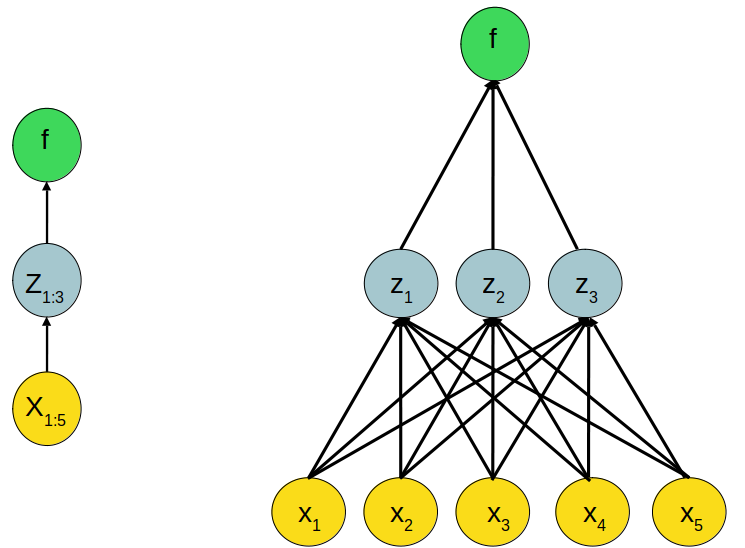
\includegraphics{figure/ffwd.png}}
      \caption{\footnotesize{Two equivalent visualizations of a dense net with a single hidden layer, the left more abstract, showing the network from a layer point-of-view.}}
  \end{figure}
\end{frame}

\begin{frame} {RNNs --- Introduction}
  \begin{itemize}
    \item Because sentences can be of varying lengths, we need to modify the dense net architecture to handle such a scenario.
    \item One approach draws inspiration from how a human reads a sentence: one word at a time.
    \item An important cognitive mechanism that makes this possible is \enquote{\textbf{short-term memory}}.
    \item As we read a sentence, we retain some information about the words already read and use this to understand the meaning of the entire sentence.
    \item Therefore, to feed the words in a sentence sequentially to a neural network, we need to give it the ability to retain some information about past inputs.
  \end{itemize}
\end{frame}

\begin{frame} {RNNs --- Introduction}
  \begin{itemize}
    \item When words in a sentence are fed to the network one at a time, the inputs are no longer independent: it is much more likely that \enquote{good} is followed by \enquote{morning} than by \enquote{plastic}. We need to model this \textbf{(long-term) dependency}.
    \item Each word must still be encoded as a fixed-length vector, because the input layer size stays fixed.
    \item Here, for visualization, each word is a one-hot vector of length 5 (\texttt{<eos>} = end of sequence).
    \begin{figure}
      \centering
      \scalebox{0.55}{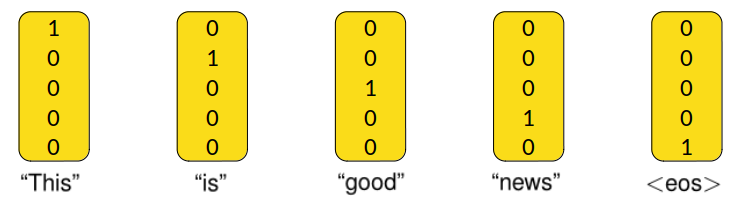
\includegraphics{figure/one_hot_1.png}}
  \end{figure}
    While this is one option, the standard approach is word embeddings (more on this later).
  \end{itemize}
\end{frame}

\begin{frame} {RNNs --- Introduction}
  \begin{itemize}
    \item Our goal is to feed the words to the network sequentially, in discrete time-steps.
    \item A regular dense network with a single hidden layer has two sets of weights: input-to-hidden weights $\mathbf{W}$ and hidden-to-output weights $\mathbf{U}$.
  \end{itemize}
  \begin{figure}
      \centering
      \scalebox{0.7}{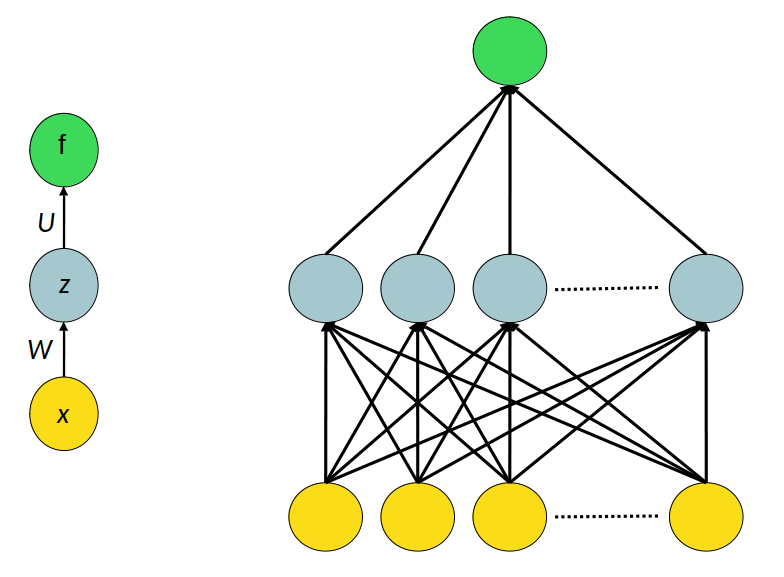
\includegraphics{figure/ffwd1.png}}
  \end{figure}
\end{frame}

\begin{frame} {RNNs --- Introduction}
  \begin{itemize}
    \item \small{To let the network retain information about past inputs, we introduce an \textbf{additional set of weights} $\mathbf{V}$, from the hidden neurons at time-step $t$ to the hidden neurons at time-step $t+1$.
    \item This makes the hidden layer's activations depend on \textbf{both} the current input and the activations for the \textit{previous} input.}
  \end{itemize}
  \begin{figure}
      \centering
      \scalebox{0.80}{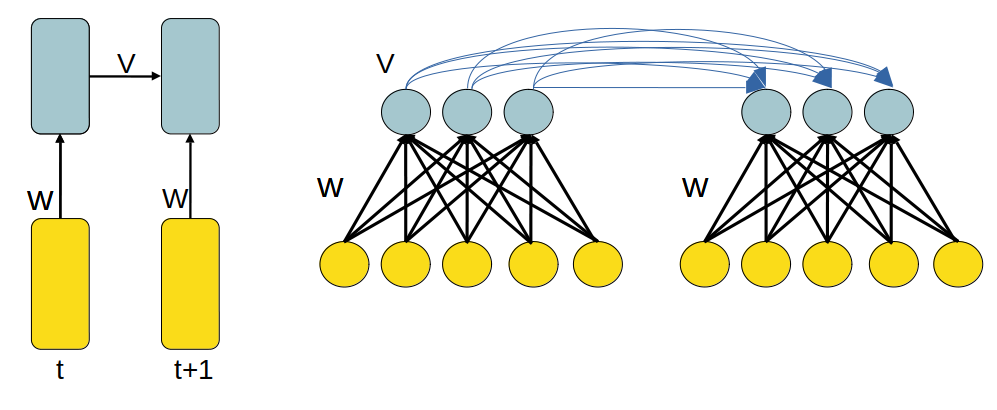
\includegraphics{figure/hidrohid.png}}
      \caption{\footnotesize Input-to-hidden weights $\mathbf{W}$ and \textbf{hidden-to-hidden} weights $\mathbf{V}$. Hidden-to-output weights $\mathbf{U}$ are omitted for readability.}
  \end{figure}
\end{frame}

\begin{frame} {RNNs --- Introduction}
  \begin{itemize}
    \item With this additional set of hidden-to-hidden weights $\mathbf{V}$, the network is now a Recurrent Neural Network (RNN).
    \item In a regular feedforward network, the hidden layer's activations only use the input-hidden weights $\mathbf{W}$ (and bias $\mathbf{b}$): $$\mathbf{z}= \sigma(\mathbf{W}^\top \xv + \mathbf{b})$$
    \item In an RNN, the activations at time-step $t$ use \textit{both} $\mathbf{W}$ and $\mathbf{V}$: $$\mathbf{z}^{[t]} = \sigma(\mathbf{\textcolor{red}{\mathbf{V}^\top\mathbf{z}^{[t-1]}}} + \mathbf{W}^\top \mathbf{x}^{[t]} + \mathbf{b})$$
    \item $\mathbf{z}^{[t]}$ represents the RNN's short-term memory: a function of the current input $\mathbf{x}^{[t]}$ and the previous activations $\mathbf{z}^{[t-1]}$.
    \item By recurrence, it contains a \enquote{summary} of \textit{all} previous inputs.
  \end{itemize}
\end{frame}

\section{RNN: Worked Example and Use Cases}

\begin{frame} {Application Example --- Sentiment Analysis}
  \begin{itemize}
    \item At $t = 0$, we feed the word \enquote{This} to the network and obtain $\mathbf{z}^{[0]}$.
    \item $\mathbf{z}^{[0]} = \sigma(\mathbf{W}^\top \mathbf{x}^{[0]} + \mathbf{b})$
  \end{itemize}
  \begin{figure}
      \centering
      \scalebox{0.48}{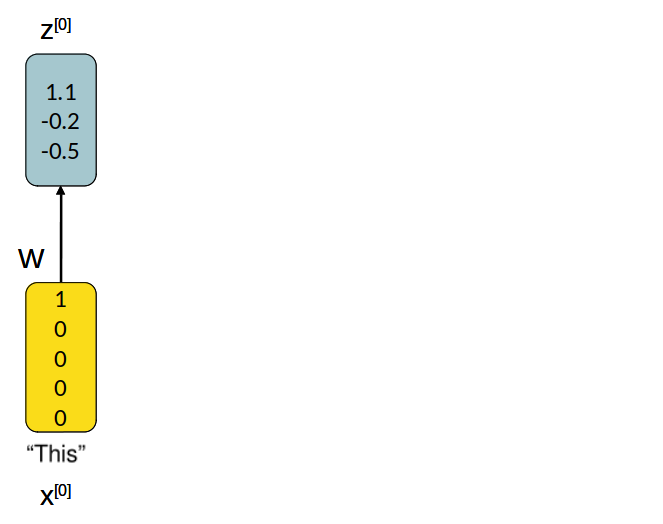
\includegraphics{figure/rnn_sample_z0.png}}
  \end{figure}
  \small{Because this is the first input, there is no past state (equivalently, the state is initialized to 0).}
\end{frame}

\begin{frame} {Application Example --- Sentiment Analysis}
  \begin{itemize}
    \item At $t = 1$, we feed the second word to obtain $\mathbf{z}^{[1]}$.
    \item $\mathbf{z}^{[1]} = \sigma(\mathbf{V}^\top\textcolor{red}{\mathbf{z}^{[0]}} + \mathbf{W}^\top \xv^{[1]} + \mathbf{b})$
  \end{itemize}
  \begin{figure}
      \centering
      \scalebox{0.55}{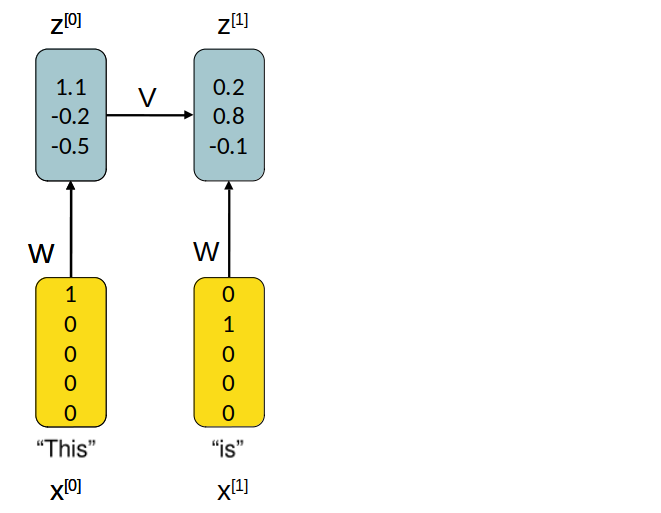
\includegraphics{figure/rnn_sample_z1.png}}
  \end{figure}
\end{frame}

\begin{frame} {Application Example --- Sentiment Analysis}
  \begin{itemize}
    \item At $t = 2$, we feed the next word.
    \item $\mathbf{z}^{[2]} = \sigma(\mathbf{V}^\top\textcolor{red}{\mathbf{z}^{[1]}} + \mathbf{W}^\top \xv^{[2]} + \mathbf{b})$
  \end{itemize}
  \begin{figure}
      \centering
      \scalebox{0.55}{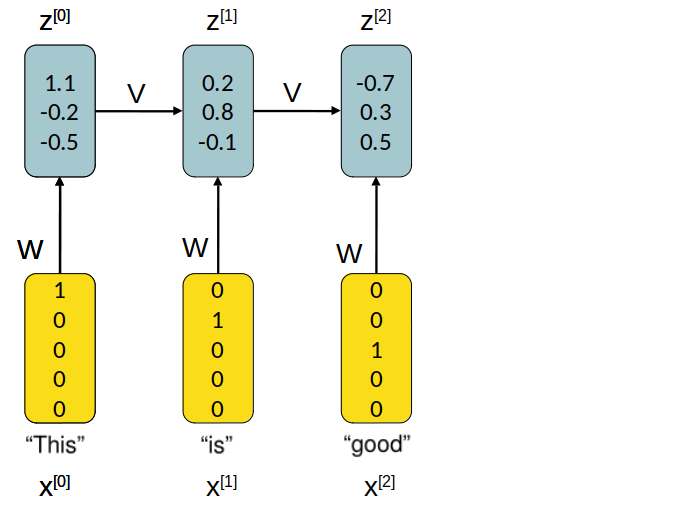
\includegraphics{figure/rnn_sample_z2.png}}
  \end{figure}
\end{frame}

\begin{frame} {Application Example --- Sentiment Analysis}
  \begin{itemize}
    \item At $t = 3$, we feed the next word (\enquote{news}).
    \item $\mathbf{z}^{[3]} = \sigma(\mathbf{V}^\top\textcolor{red}{\mathbf{z}^{[2]}} + \mathbf{W}^\top \xv^{[3]} + \mathbf{b})$
  \end{itemize}
  \begin{figure}
      \centering
      \scalebox{0.65}{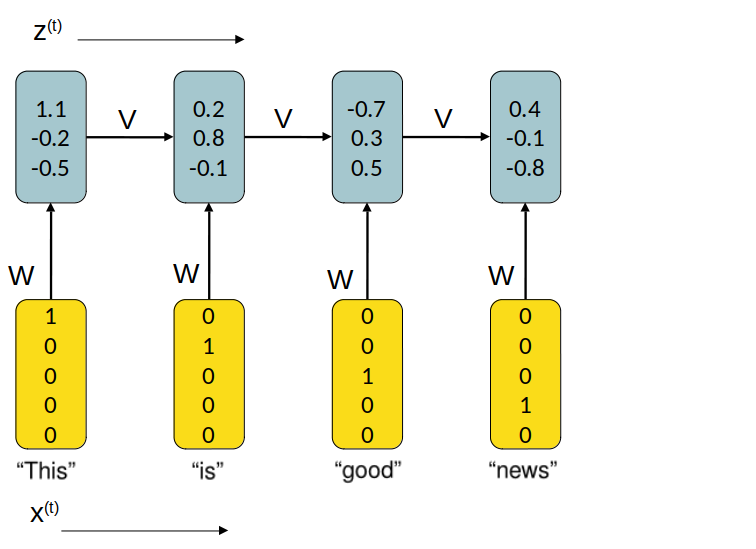
\includegraphics{figure/rnn_sample_z3.png}}
  \end{figure}
\end{frame}

\begin{frame} {Application Example --- Sentiment Analysis}
  \begin{itemize}
    \item Once the entire sequence has been processed, the prediction is generated by feeding the final time-step's activations to the output neuron(s).
    \item $f = \sigma (\mathbf{U}^\top \mathbf{z}^{[4]} + {c})$, where $c$ is the output neuron's bias.
  \end{itemize}
  \begin{figure}
      \centering
      \scalebox{0.48}{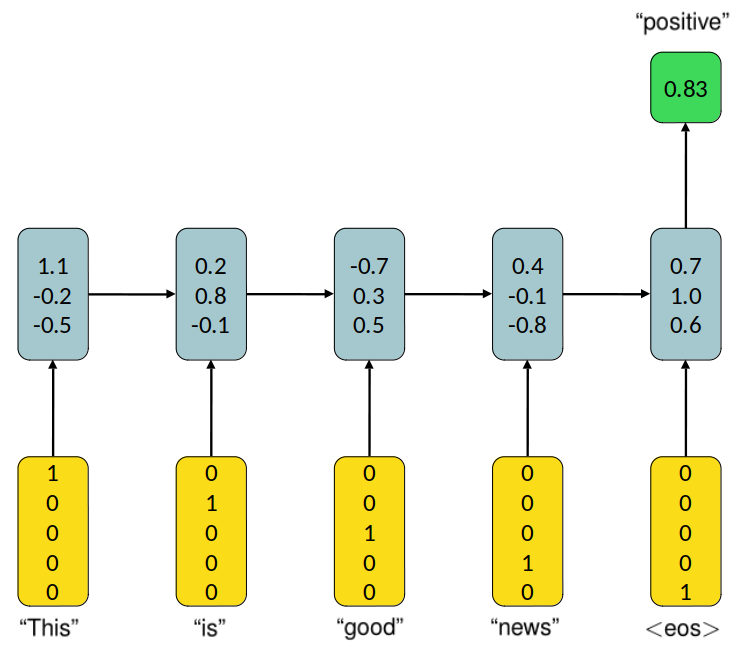
\includegraphics{figure/rnn_sample_z5.png}}
  \end{figure}
\end{frame}

\begin{frame} {Parameter Sharing}
  \begin{itemize}
    \item This way, the network processes the sentence one word at a time, and its length can vary based on the sequence length.
    \item No matter how long the input sequence is, the matrices $\mathbf{W}$ and $\mathbf{V}$ are the \textbf{same} at every time-step --- another example of \textbf{parameter sharing} (recall this idea from CNNs, Session 5).
    \item Therefore, the number of weights in the network is independent of the input sequence length.
  \end{itemize}
\end{frame}

\begin{frame} {RNNs --- Use-Case-Specific Architectures}
  \small{RNNs are very versatile and apply to a wide range of tasks.
  \begin{figure}
      \centering
      \scalebox{0.9}{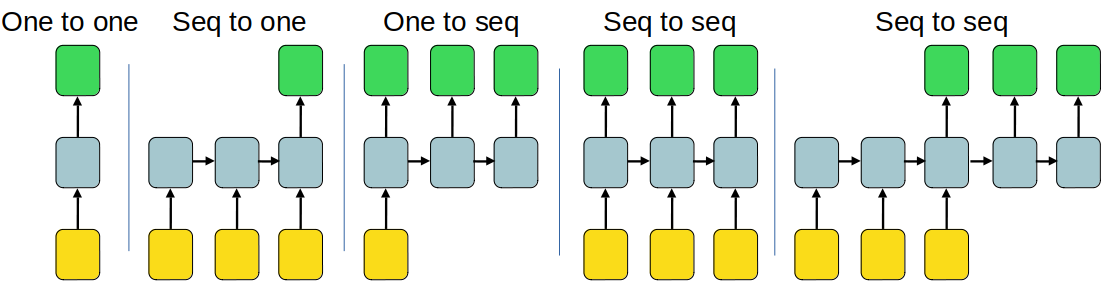
\includegraphics{figure/one_to_one.png}}
      \caption{\footnotesize {RNNs can be used in tasks with multiple inputs and/or multiple outputs.}}
  \end{figure}
  Examples:}
  \begin{itemize}
    \item \small{Sequence-to-One: sentiment analysis, document classification.
    \item One-to-Sequence: image captioning.
    \item Sequence-to-Sequence: language modelling, machine translation, time-series prediction.}
  \end{itemize}
\end{frame}

%%%%%%%%%%%%%%%%%%%%%%%%%%%%%%%%%%%%%%%%%%%%%%%%%%%%%%%%%%%%%%%%%%
\section{RNN: Computational Graph and Bidirectional RNNs}
%%%%%%%%%%%%%%%%%%%%%%%%%%%%%%%%%%%%%%%%%%%%%%%%%%%%%%%%%%%%%%%%%%

\frame{
\frametitle{RNNs --- Computational Graph}
  \center
  \begin{figure}%
    \only<1>{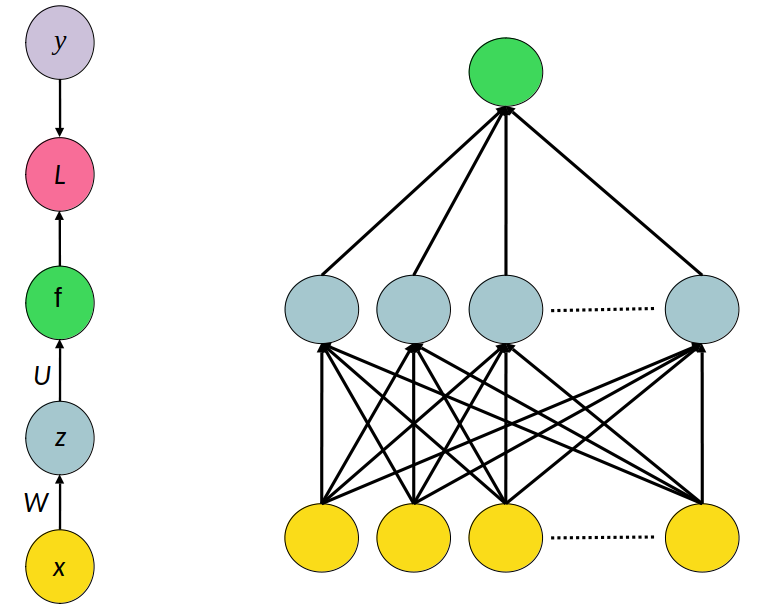
\includegraphics[width=7cm]{figure/nonrecurrent.png}}%
    \only<2>{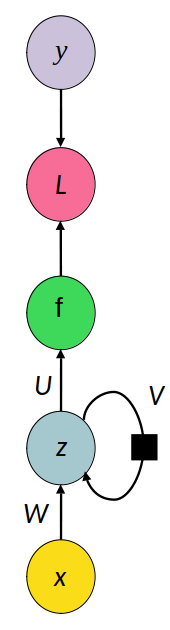
\includegraphics[width=1.5cm]{figure/recurrent_single.png}}%
    \only<3-4>{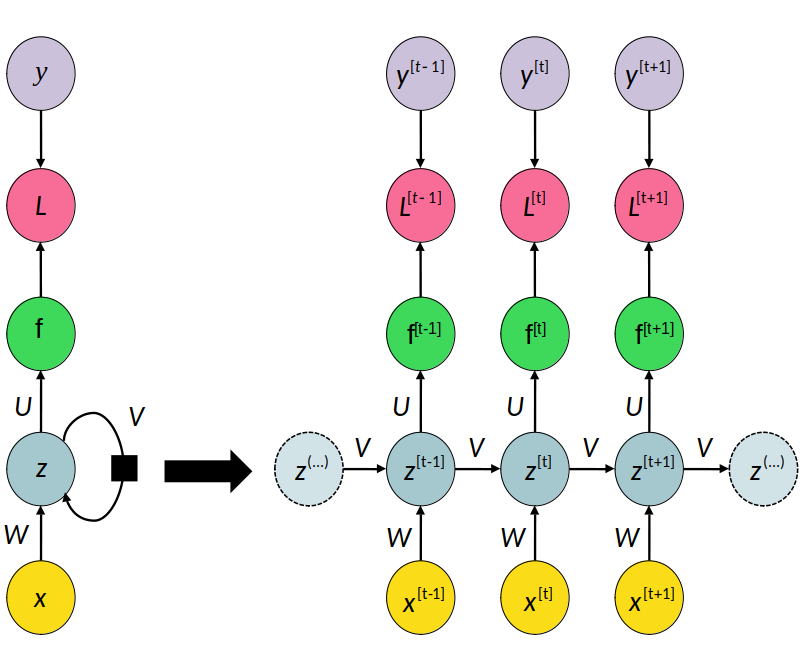
\includegraphics[width=7cm]{figure/recurrent_unfolded.png}}%
    \only<5>{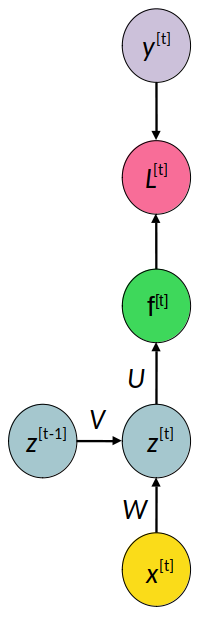
\includegraphics[width=1.5cm]{figure/rnn_zt_figure.png}}%
  \end{figure}%
  \vspace{-0.2cm}
  \begin{itemize}
    \only<1>{\item On the left, an abstract representation of the computational graph for the network on the right. A loss $L$ measures how far each output $f$ is from the training target $y$.}
    \only<2>{\item A helpful way to think of an RNN: multiple copies of the same network, each passing a message to a successor.}
    \only<2>{\item RNNs are networks with loops, allowing information to persist.}
    \only<3>{\item Things become clearer if we unfold the architecture.}
    \only<3>{\item We call $\mathbf{z}^{[t]}$ the \textit{state} of the system at time $t$.}
    \only<3>{\item The state contains information about the whole past sequence.}
    \only<4>{\item We went from
      \begin{eqnarray*}
        f &=& \tau(c + \mathbf{U}^\top \sigma(\mathbf{b} + \mathbf{W}^\top \mathbf{x})) \text{ for the dense net, to } \\
        f^{[t]} &=& \tau(c + \mathbf{U}^\top \sigma(\mathbf{b} + \mathbf{V}^\top \mathbf{z}^{[t-1]} + \mathbf{W}^\top \xv^{[t]})) \text{ for the RNN. }
      \end{eqnarray*}}
    \only<5>{\item A potential computational graph for time-step $t$ with}
    \only<5>{\item[] $$f^{[t]} = \tau(c + \mathbf{U}^\top \sigma(\mathbf{b} + \mathbf{V}^\top \mathbf{z}^{[t-1]} + \mathbf{W}^\top \xv^{[t]})) $$ }
  \end{itemize}
}

\frame{
\frametitle{Recurrent Output-Hidden Connections}
Recurrent connections do not need to map from hidden to hidden neurons!
\center
\begin{figure}
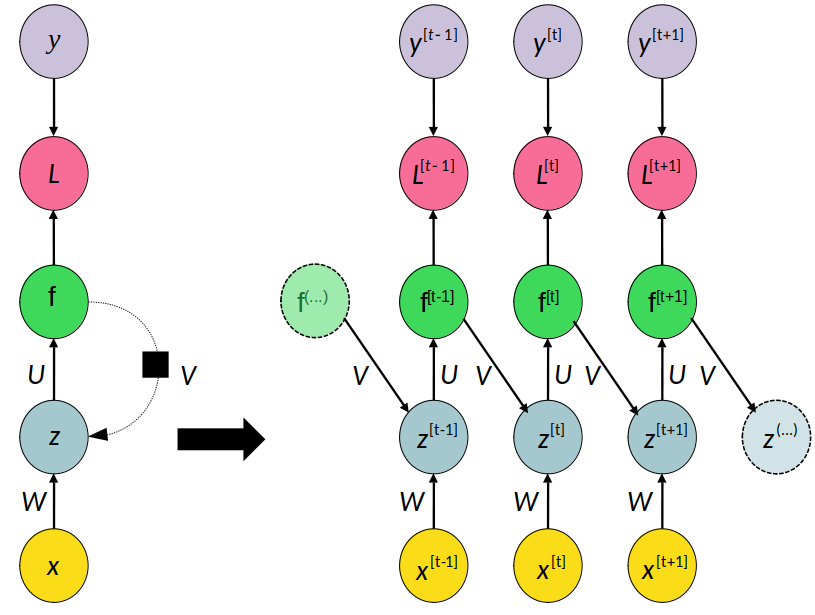
\includegraphics[width=5.5cm]{figure/recurrent_unfolded_fromoutput.png}
\caption{\footnotesize RNN with feedback connection from the output to the hidden layer. The RNN may only send $f$ to future time points, so $z^{[t-1]}$ is connected to $z^{[t]}$ only indirectly, via the predictions $f^{[t-1]}$.}
\end{figure}
}

\frame{
\frametitle{Seq-to-One Mappings}
RNNs do not need to produce an output at each time step --- often only one output is produced after processing the whole sequence.
\center
\begin{figure}
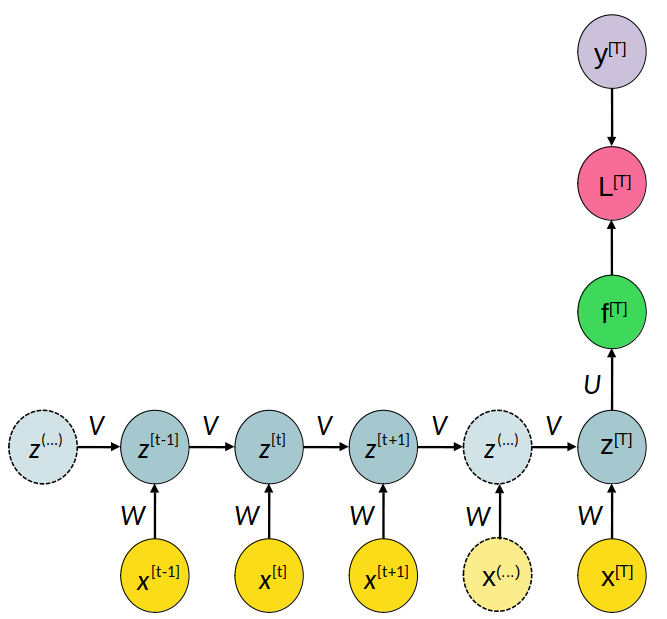
\includegraphics[width=5cm]{figure/rnn_last_output.png}
     \caption{Time-unfolded RNN with a single output at the end of the sequence. Such a network can summarize a sequence into a fixed-size representation.}
\end{figure}
}

\begin{vbframe}{Bidirectional RNNs}
  \begin{itemize}
    \item A generalization of the simple RNN.
    \item Allows processing sequential data depending on both past and future inputs --- e.g.\ predicting missing words, which likely depend on both preceding and following words.
    \item One RNN processes inputs forward, from $\mathbf{x}^{[1]}$ to $\mathbf{x}^{[T]}$, computing hidden states $(\mathbf{z}^{[1]}, \dots, \mathbf{z}^{(T)})$; another processes backward, from $\mathbf{x}^{[T]}$ to $\mathbf{x}^{[1]}$, computing $(\mathbf{g}^{[T]}, \dots, \mathbf{g}^{[1]})$.
    \item Predictions are based on both hidden states (e.g.\ by concatenation).
    \item With connections going back in time, the whole input sequence must be known in advance to train and infer from the model.
    \item Often used for the encoding of a sequence in machine translation.
  \framebreak
\textbf{Computational graph of a bidirectional RNN:}
  \begin{figure}
    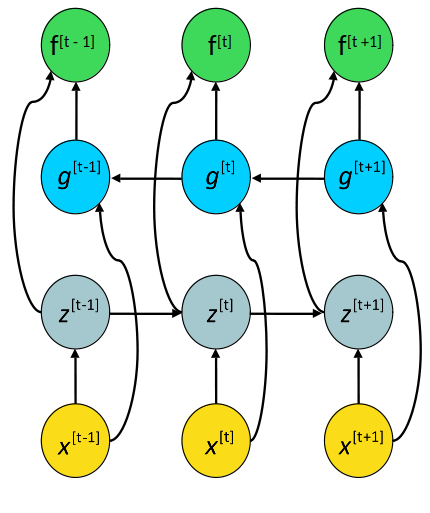
\includegraphics[width=4.5cm]{figure/bidirectional_rnn.png}
    \caption{A bidirectional RNN: a forward RNN processing inputs left to right, and a backward RNN processing inputs backwards in time.}
  \end{figure}
  \end{itemize}
\end{vbframe}

\begin{vbframe}{Multi-Layer (Stacked) RNNs}
  \begin{itemize}
    \item A stack of several RNNs (vanilla RNNs, LSTMs, GRUs, \ldots), each with its own parameters.
    \item The input vectors of the $l$-th RNN in the stack are the hidden states of the $(l-1)$-th RNN; the first RNN's inputs are the word embeddings, as usual.
    \item We can output the hidden states of the last RNN, or a combination (concatenation, average, \ldots) of the states of all RNNs.
    \item Stacking adds representational capacity, analogous to adding depth in a feedforward or convolutional net.
  \end{itemize}
  \begin{center}
  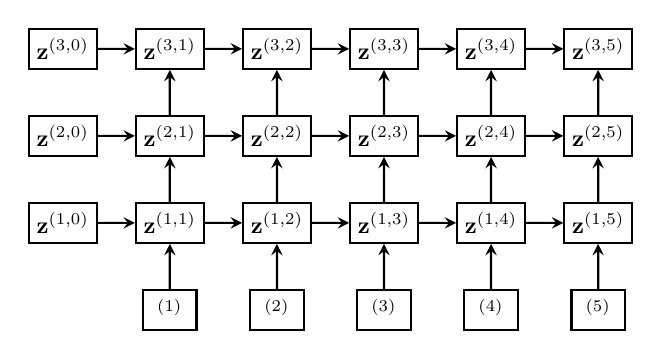
\begin{tikzpicture}[->, thick, >=stealth, scale=0.85, every node/.style={scale=0.85}]
  \tikzstyle{vecbox}=[draw, rectangle, minimum width=8mm, minimum height=6mm]
  \node (h10) [vecbox] at (0,1.3) {$\mathbf{z}^{(1,0)}$};
  \node (h20) [vecbox] at (0,2.6) {$\mathbf{z}^{(2,0)}$};
  \node (h30) [vecbox] at (0,3.9) {$\mathbf{z}^{(3,0)}$};
  \foreach \i in {1,...,5}{
  \node (x\i) [vecbox] at (\i*1.6,0) {$\xv^{(\i)}$};
  \node (h1\i) [vecbox] at (\i*1.6,1.3) {$\mathbf{z}^{(1,\i)}$};
  \node (h2\i) [vecbox] at (\i*1.6,2.6) {$\mathbf{z}^{(2,\i)}$};
  \node (h3\i) [vecbox] at (\i*1.6,3.9) {$\mathbf{z}^{(3,\i)}$};
  \pgfmathparse{\i-1}
  \draw (h1\pgfmathresult) -- (h1\i);
  \draw (h2\pgfmathresult) -- (h2\i);
  \draw (h3\pgfmathresult) -- (h3\i);
  \draw (x\i) -- (h1\i);
  \draw (h1\i) -- (h2\i);
  \draw (h2\i) -- (h3\i);
  }
  \end{tikzpicture}
  \end{center}
\end{vbframe}

%%%%%%%%%%%%%%%%%%%%%%%%%%%%%%%%%%%%%%%%%%%%%%%%%%%%%%%%%%%%%%%%%%
\section{RNN: Backpropagation Through Time}
%%%%%%%%%%%%%%%%%%%%%%%%%%%%%%%%%%%%%%%%%%%%%%%%%%%%%%%%%%%%%%%%%%

\begin{vbframe}{Simple Example: Character-Level Language Model}
Task: learn a character probability distribution from input text.
   \begin{itemize}
     \item Suppose our vocabulary has four letters: \enquote{h}, \enquote{e}, \enquote{l}, \enquote{o}, and we train an RNN on the sequence \enquote{hello}.
     \item This training sequence is actually a source of 4 separate training examples:
       \begin{itemize}
         \item \enquote{e} should be likely given the context of \enquote{h}
         \item \enquote{l} should be likely given the context of \enquote{he}
         \item \enquote{l} should also be likely given the context of \enquote{hel}
         \item \enquote{o} should be likely given the context of \enquote{hell}
       \end{itemize}
   \end{itemize}
\framebreak
   \begin{itemize}
     \item[] The RNN has a 4-dimensional input and output. The exemplary hidden layer has 3 neurons. This diagram shows the forward-pass activations when the RNN is fed \enquote{hell}. The output holds the RNN's confidences for the next character.
   \end{itemize}
   \begin{figure}
       \centering
       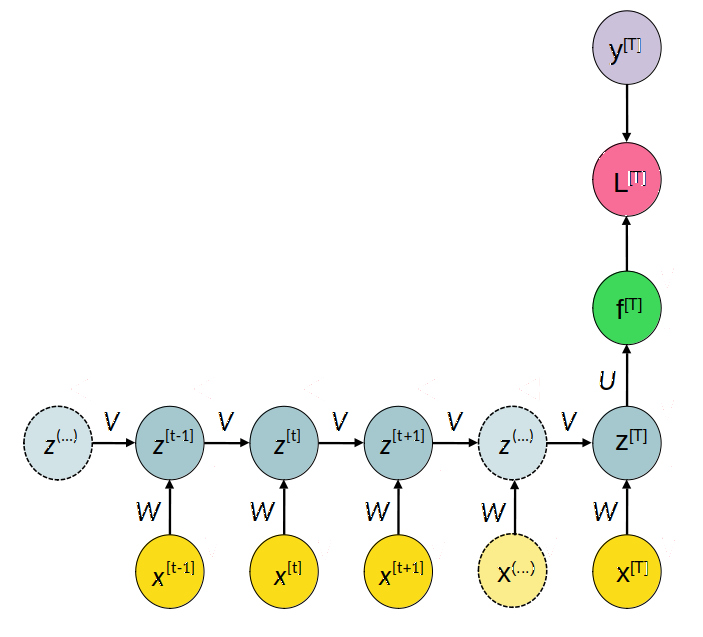
\includegraphics[width=6cm]{figure/backpropagation_rnn_forward.png}
   \end{figure}
   Our goal is to increase confidence for the correct letters and decrease it for all others (a softmax activation could squash these to probabilities). How do we train the network? \textbf{Backpropagation through time!}
\end{vbframe}

\frame{
\frametitle{Backpropagation Through Time}
  \begin{columns}[T]
    \begin{column}{0.42\textwidth}
      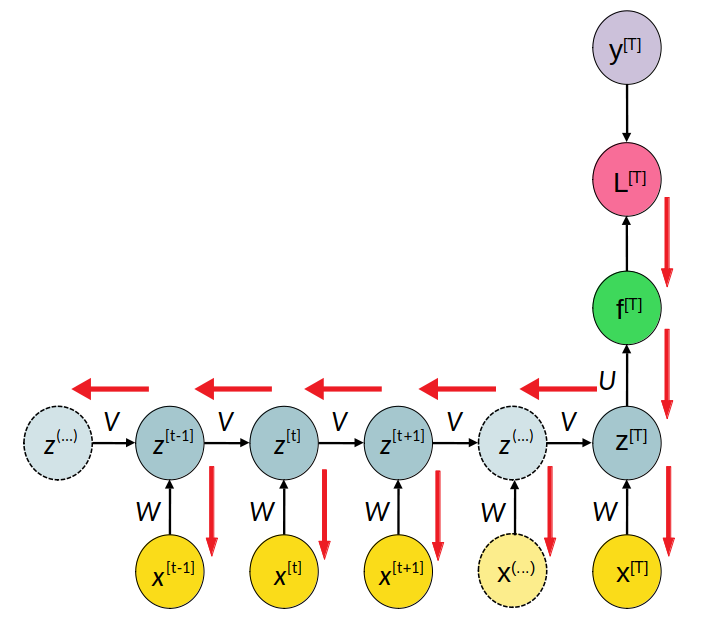
\includegraphics[width=\textwidth]{figure/backpropagation_rnn.png}
    \end{column}
    \begin{column}{0.58\textwidth}
      \begin{itemize}
        \item To train the RNN, we need $\frac{d L}{d u_{i,j}}$, $\frac{d L}{d v_{i,j}}$, and $\frac{d L}{d w_{i,j}}$.
        \item During backpropagation at time step $t$, we need to compute
        $$\frac{d L}{d \mathbf{z}^{[1]}} = \frac{d L}{d \mathbf{z}^{[t]}} \frac{d \mathbf{z}^{[t]}}{d \mathbf{z}^{[t-1]}} \dots \frac{d \mathbf{z}^{[2]}}{d \mathbf{z}^{[1]}}$$
      \end{itemize}
    \end{column}
  \end{columns}
}

\begin{vbframe}{Long-Term Dependencies}
  \begin{itemize}
    \item Here, $\mathbf{z}^{[t]} = \sigma(\mathbf{V}^\top \mathbf{z}^{[t-1]} + \mathbf{W}^\top \xv^{[t]} + \mathbf{b})$, so:
    $$ \frac{d \mathbf{z}^{[t]}}{d\mathbf{z}^{[t-1]}} = \text{diag}(\sigma' (\mathbf{V}^\top \mathbf{z}^{[t-1]} + \mathbf{W}^\top \xv^{[t]} + \mathbf{b})) \mathbf{V}^\top = \mathbf{D}^{[t-1]} \mathbf{V}^\top $$
    $$ \vdots $$
    $$ \frac{d L}{d \mathbf{z}^{[1]}} = \frac{d L}{d \mathbf{z}^{[t]}} \mathbf{D}^{[t-1]} \mathbf{D}^{[t-2]}   \text{ . . . } \mathbf{D}^{[1]} (\mathbf{V}^\top)^{t-1}$$
    \item In general, for an arbitrary past time-step $i<t$, $\frac{d\mathbf{z}^{[t]}}{d\mathbf{z}^{[i]}}$ contains the term $(\mathbf{V}^\top)^{t-i}$ (by the chain rule).
    \item Based on the largest eigenvalue of $\mathbf{V}^\top$, this term can cause vanishing or exploding gradients.
    \item This is more severe for RNNs than feedforward networks, because the \textbf{same} matrix $\mathbf{V}^\top$ is multiplied repeatedly. As the gap between $t$ and $i$ grows, the instability worsens.
    \item It is thus challenging for RNNs to learn long-term dependencies: gradients either \textbf{vanish} (usually) or \textbf{explode} (rarely, but destructively) simply because errors propagate over very many stages.
  \end{itemize}
  \begin{itemize}
    \item We can counteract exploding gradients with gradient clipping: clip the gradient norm at some threshold $h$: $$\text{if  } ||\nabla W|| > \text h: \nabla W \leftarrow \frac{h}{||\nabla W||} \nabla W $$
  \end{itemize}
  \begin{itemize}
    \item Even for a stable RNN, long-term interactions get exponentially smaller weights than short-term ones --- a more sophisticated fix is needed for vanishing gradients (next: LSTM, GRU).
    \item The vanishing gradient problem heavily depends on the activation function: sigmoid squashes into $[0,1]$, so even large input changes yield small output changes, and gradients shrink further when layers stack. ReLU avoids this (gradients are $0$ or $1$, never saturating) at the cost of possible \enquote{dead} units.
  \end{itemize}
\end{vbframe}

%%%%%%%%%%%%%%%%%%%%%%%%%%%%%%%%%%%%%%%%%%%%%%%%%%%%%%%%%%%%%%%%%%
\section{LSTM and GRU}
%%%%%%%%%%%%%%%%%%%%%%%%%%%%%%%%%%%%%%%%%%%%%%%%%%%%%%%%%%%%%%%%%%

\frame{
\frametitle{Long Short-Term Memory (LSTM)}
The LSTM provides a way of dealing with vanishing gradients and modelling long-term dependencies.
  \begin{figure}
    \only<1>{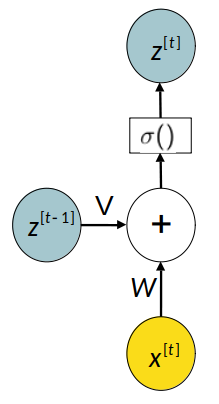
\includegraphics[width=2cm]{figure/vanilla_rnn.png}}%
    \only<2>{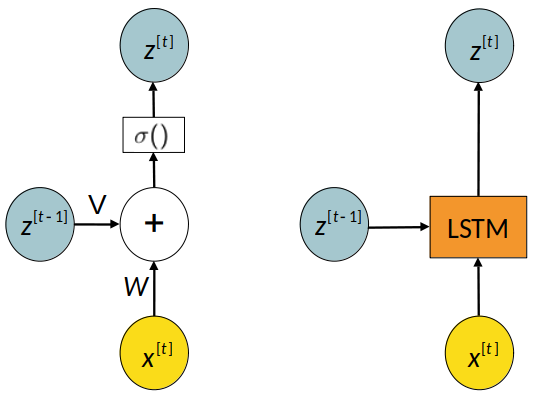
\includegraphics[width=5cm]{figure/vanilla_rnn_lstm.png}}%
\tiny{\\\only<2>{Left:} A simple RNN mechanism; \only<2>{Right: An LSTM cell}}
  \end{figure}
  \begin{itemize}
    \only<1-2>{\item Until now, we simply computed $$\mathbf{z}^{[t]} = \sigma(\mathbf{b} + \mathbf{V}^\top \mathbf{z}^{[t-1]} + \mathbf{W}^\top \xv^{[t]})$$}
    \only<2>{\item Now we introduce the LSTM cell, a small network on its own.}
  \end{itemize}
}

\frame{
\frametitle{Long Short-Term Memory (LSTM)}
  \center
  \only<1>{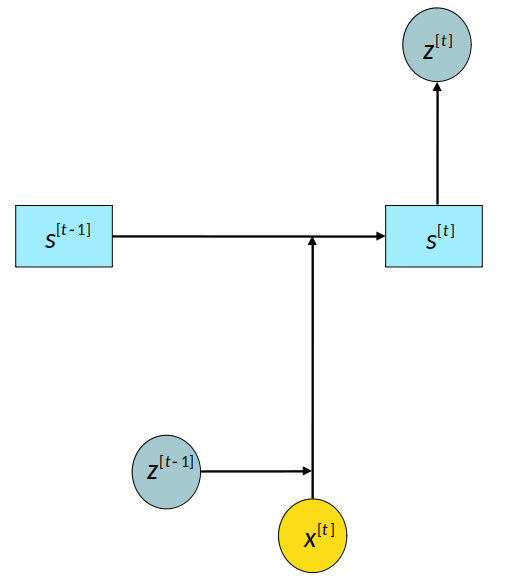
\includegraphics[width=3.5cm]{figure/lstm_1.png}}%
  \only<2>{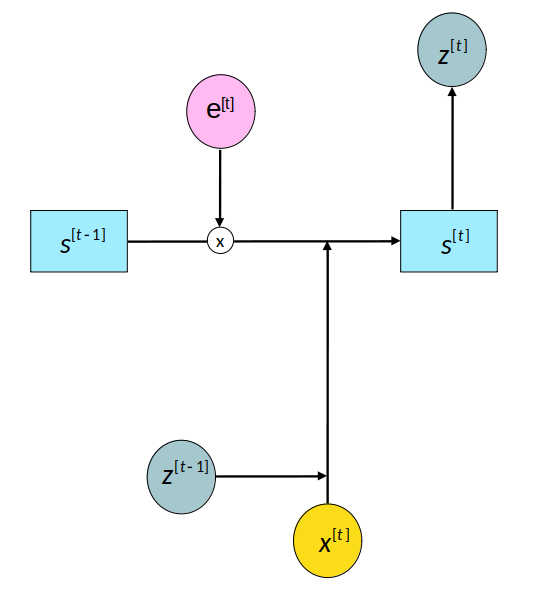
\includegraphics[width=3.5cm]{figure/lstm_2.png}}%
  \only<3-4>{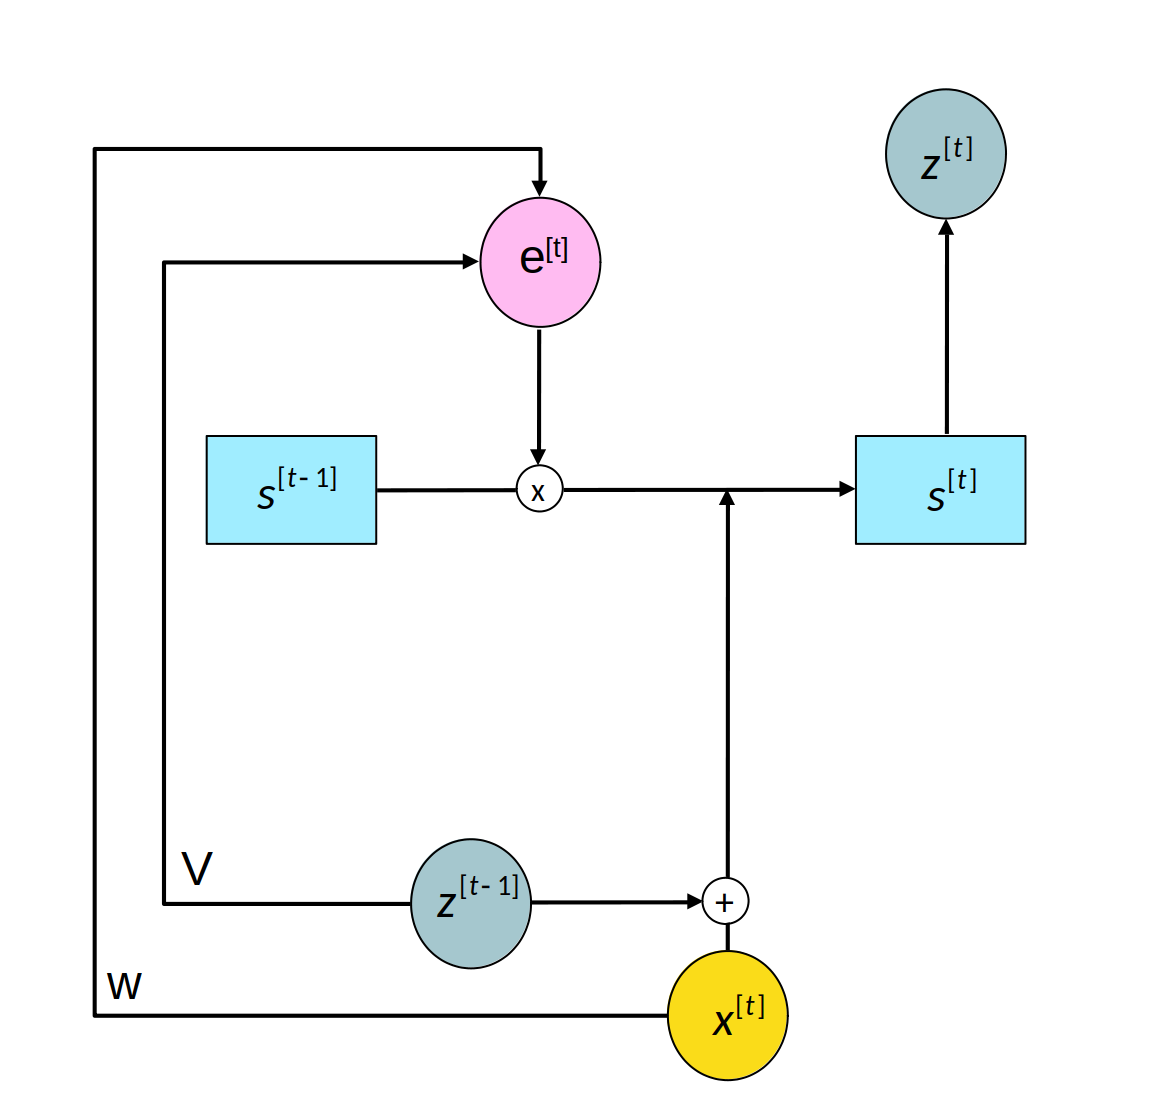
\includegraphics[width=4.75cm]{figure/lstm_3.png}}%
  \only<5-7>{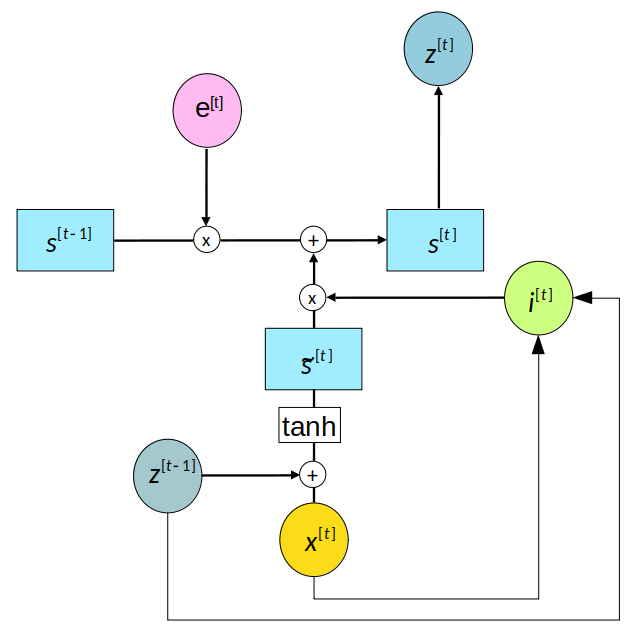
\includegraphics[width=4.75cm]{figure/lstm_4.png}}%
  \only<8-9>{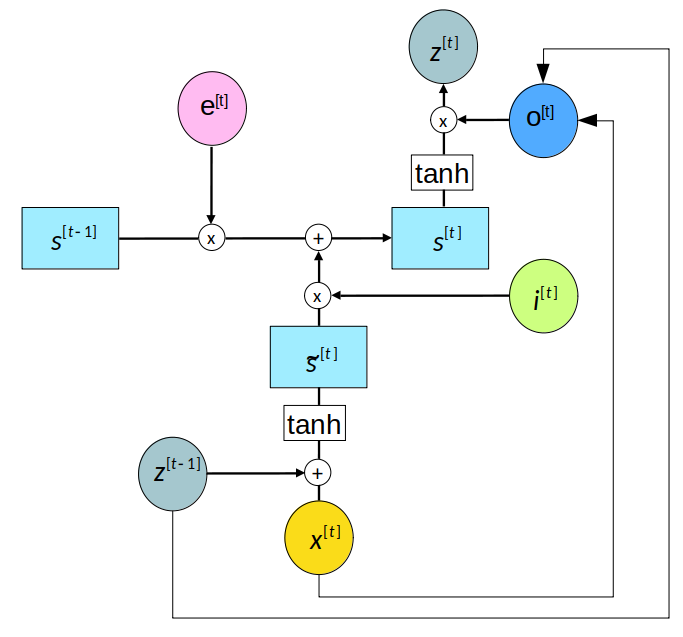
\includegraphics[width=4.75cm]{figure/lstm_5.png}}%
  \begin{itemize}
    \only<1>{\item The key to LSTMs is the \textbf{cell state} $\mathbf{s}^{[t]}$.}
    \only<1>{\item $\mathbf{s}^{[t]}$ can be manipulated by different \textbf{gates} to forget old information, add new information, and read information out of it.}
    \only<1>{\item Each gate is a vector the size of $\mathbf{s}^{[t]}$, with elements between 0 (\enquote{let nothing pass}) and 1 (\enquote{let everything pass}).}
    \only<2>{\item \textbf{Forget gate} $\mathbf{e}^{[t]}$: indicates which information of the old cell state we should forget.
    \item Intuition: a model predicting the next word might track the subject's gender for pronoun agreement. On seeing a new subject, we want to forget the old gender.}
    \only<3>{\item We obtain the forget gate via
    $$\mathbf{e}^{[t]} = \sigma(\mathbf{b}_{e} + \mathbf{V}_e^\top \mathbf{z}^{[t-1]} + \mathbf{W}_e^\top \xv^{[t]})$$}
    \only<3>{\item $\sigma()$ is a sigmoid, $\mathbf{V}_e, \mathbf{W}_e$ are forget-gate-specific weights.}
    \only<4>{\item To compute $\mathbf{s}^{[t]}$, first multiply (elementwise) the previous cell state $\mathbf{s}^{[t-1]}$ by the forget gate: $$\mathbf{e}^{[t]} \odot \mathbf{s}^{[t-1]}, \text{ with } \mathbf{e}^{[t]} \in [0,1]$$}
    \only<5>{\item \textbf{Input gate} $\mathbf{i}^{[t]}$: indicates which new information should be added to $\mathbf{s}^{[t]}$.}
    \only<5>{\item Intuition: this is where we add the new subject's gender.}
    \only<6>{\item The new information is $\tilde{\mathbf{s}}^{[t]} = \text{tanh}(\mathbf{b} + \mathbf{V}^\top \mathbf{z}^{[t-1]} + \mathbf{W}^\top \xv^{[t]}) \in [-1, 1]$.}
    \only<6>{\item The input gate is $\mathbf{i}^{[t]} = \sigma(\mathbf{b}_i + \mathbf{V}_i^\top \mathbf{z}^{[t-1]} + \mathbf{W}_i^\top \xv^{[t]}) \in [0,1]$.}
   \only<6>{\item $\mathbf{W}, \mathbf{V}$ are the new-information weights; $\mathbf{W}_i, \mathbf{V}_i$ the input-gate weights.}
    \only<7>{\item Now we can compute the cell state $\mathbf{s}^{[t]}$:
    $$\mathbf{s}^{[t]} = \mathbf{e}^{[t]} \odot \mathbf{s}^{[t-1]} + \mathbf{i}^{[t]} \odot \tilde{\mathbf{s}}^{[t]}$$}
    \only<8>{\item \textbf{Output gate} $\mathbf{o}^{[t]}$: indicates which information from the cell state is filtered out.
   \item $\mathbf{o}^{[t]} = \sigma(\mathbf{b}_o + \mathbf{V}_o^\top \mathbf{z}^{[t-1]} + \mathbf{W}_o^\top \xv^{[t]})$, with specific weights $\mathbf{W}_o, \mathbf{V}_o$.}
    \only<9>{\item Finally, the new state $\mathbf{z}^{[t]}$ is a function of the cell state, multiplied by the output gate: $$\mathbf{z}^{[t]} = \mathbf{o}^{[t]} \odot \text{tanh}(\mathbf{s}^{[t]})$$}
  \end{itemize}
}

\frame{
\frametitle{Gated Recurrent Units (GRU)}
   \begin{itemize}
     \item The key distinction from regular RNNs: GRUs support gating of the hidden state.
     \item Dedicated mechanisms decide when a hidden state should be updated, and when it should be reset.
     \item These mechanisms are learned to:
     \begin{itemize}
           \item avoid the vanishing/exploding gradient problem of a standard RNN,
           \item using an update gate and a reset gate,
           \item that control information flowing into (update gate) and out of (reset gate) memory.
     \end{itemize}
   \end{itemize}
}

\begin{vbframe}{Gated Recurrent Units (GRU)}
    \begin{figure}
      \centering
      \scalebox{0.38}{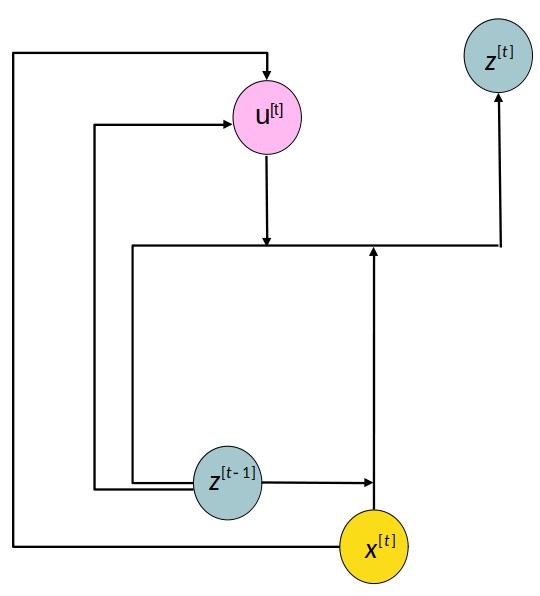
\includegraphics{figure/gru_1.png}}
      \caption{\footnotesize{Update gate in a GRU.}}
  \end{figure}
  \begin{itemize}
    \item For time step $t$, the hidden state of the last time step is $\mathbf{z}^{[t-1]}$. The update gate $\mathbf{u}^{[t]}$ is:
   \item $\mathbf{u}^{[t]} = \sigma(\mathbf{W}_{u}^\top \mathbf{x}^{[t]} + \mathbf{V}_{u}^\top \mathbf{z}^{[t-1]}  + \mathbf{b}_u)$
    \item We use a sigmoid to transform input values to $(0,1)$.
  \end{itemize}
\end{vbframe}

\begin{vbframe}{Gated Recurrent Units (GRU)}
    \begin{figure}
      \centering
      \scalebox{0.4}{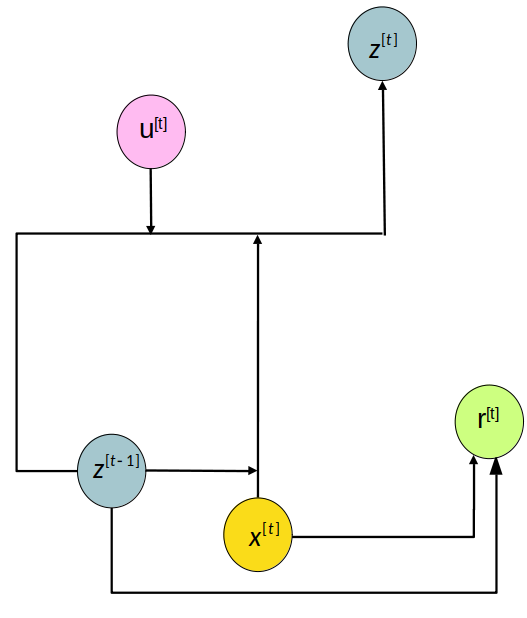
\includegraphics{figure/gru_2.png}}
      \caption{\footnotesize{Reset gate in a GRU.}}
  \end{figure}
  \begin{itemize}
    \item Similarly, the reset gate $\mathbf{r}^{[t]}$ is:
   \item $\mathbf{r}^{[t]} = \sigma(\mathbf{W}_{r}^\top \mathbf{x}^{[t]} +\mathbf{V}_{r}^\top \mathbf{z}^{[t-1]} + \mathbf{b}_r)$
  \end{itemize}
\end{vbframe}

\begin{vbframe}{Gated Recurrent Units (GRU)}
     \begin{figure}
      \centering
      \scalebox{0.4}{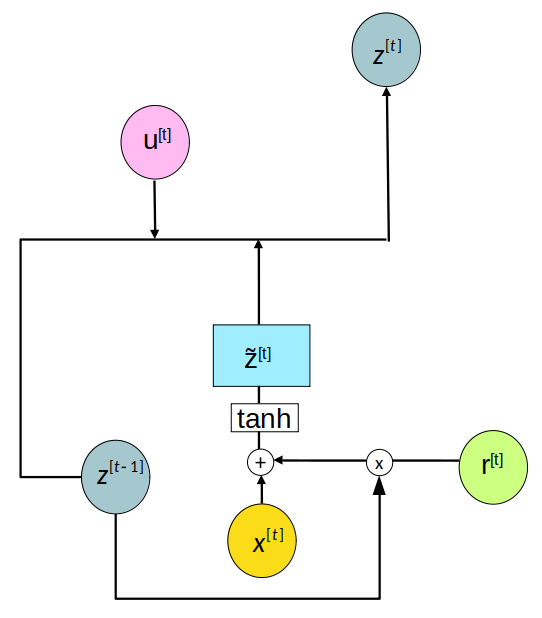
\includegraphics{figure/gru_25.png}}
      \caption{\footnotesize{Hidden state computation in a GRU (elementwise multiplication).}}
  \end{figure}
  \begin{itemize}
  \item  $\tilde{\mathbf{z}}^{[t]} = \tanh(\mathbf{W}_{z}^\top \mathbf{x}^{[t]} + \mathbf{V}_{z}^\top \left(\mathbf{r}^{[t]} \odot \mathbf{z}^{[t-1]}\right)  + \mathbf{b}_z).$
   \item In a conventional RNN, the hidden state update would instead be: $\mathbf{z}^{[t]} = \tanh(\mathbf{W}_{z}^\top \mathbf{x}^{[t]} + \mathbf{V}_{z}^\top \mathbf{z}^{[t-1]} + \mathbf{b}_z).$
   \end{itemize}
\end{vbframe}

\begin{vbframe}{Gated Recurrent Units (GRU)}
 \begin{figure}
      \centering
      \scalebox{0.4}{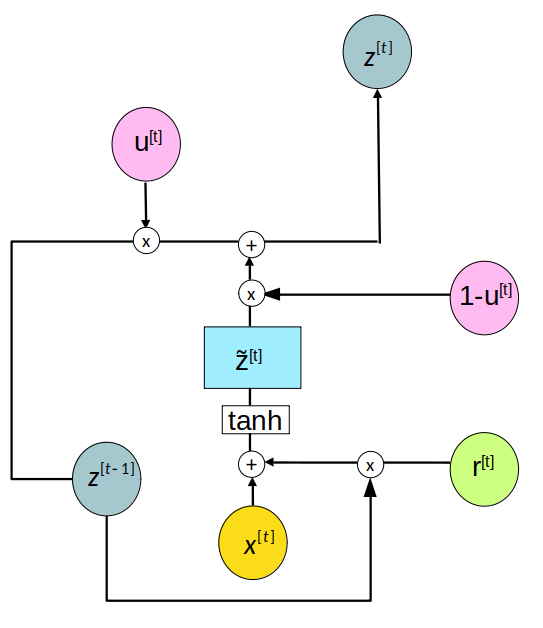
\includegraphics{figure/gru_3.png}}
      \caption{\footnotesize{Update gate in a GRU (elementwise multiplication).}}
  \end{figure}
  \begin{itemize}
  \item The update gate $\mathbf{u}^{[t]}$ determines how much of the old state $\mathbf{z}^{[t-1]}$ and the new candidate state $\tilde{\mathbf{z}}^{[t]}$ is used:
  \item $\mathbf{z}^{[t]} = \mathbf{u}^{[t]} \odot \mathbf{z}^{[t-1]}  + (1 - \mathbf{u}^{[t]}) \odot \tilde{\mathbf{z}}^{[t]}.$
  \end{itemize}
  These designs help eliminate the vanishing gradient problem in RNNs and capture dependencies over larger time-step distances. In summary, GRUs have two distinguishing features:
  \begin{itemize}
    \item Reset gates help capture short-term dependencies.
    \item Update gates help capture long-term dependencies.
  \end{itemize}
\end{vbframe}

\begin{vbframe}{GRU vs.\ LSTM}
  \begin{figure}
     \centering
      \scalebox{0.8}{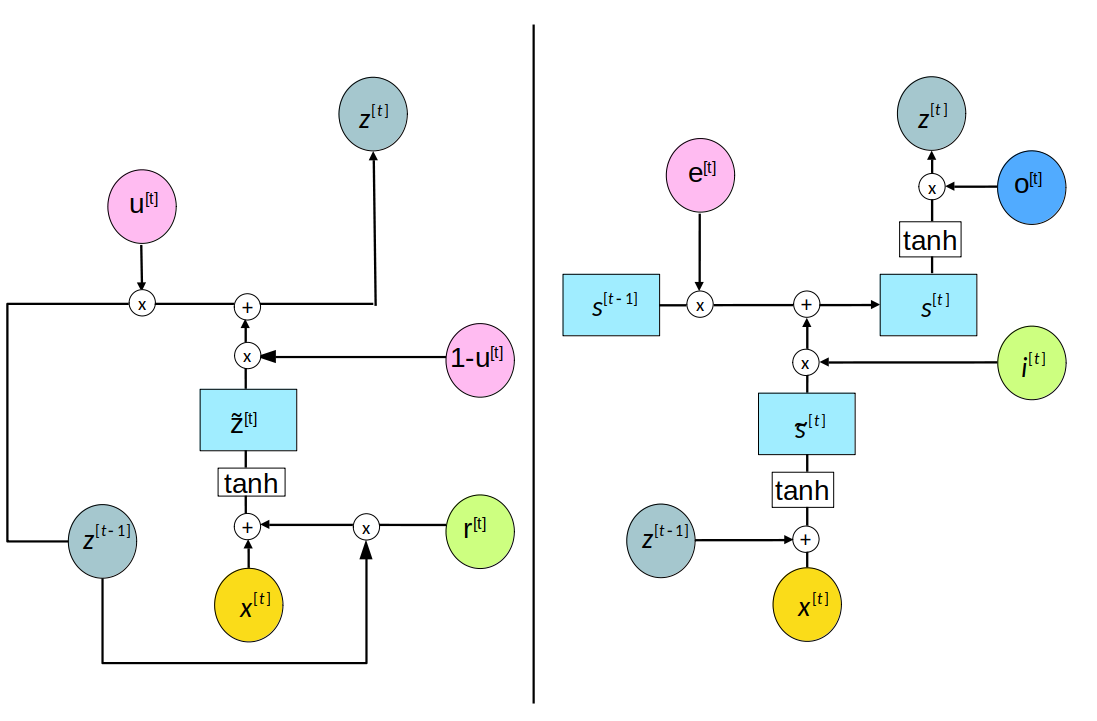
\includegraphics{figure/gru_vs_lstm.png}}
      \caption{\footnotesize{GRU vs.\ LSTM}}
  \end{figure}
\end{vbframe}

%%%%%%%%%%%%%%%%%%%%%%%%%%%%%%%%%%%%%%%%%%%%%%%%%%%%%%%%%%%%%%%%%%
\section{RNN Applications}
%%%%%%%%%%%%%%%%%%%%%%%%%%%%%%%%%%%%%%%%%%%%%%%%%%%%%%%%%%%%%%%%%%

\begin{frame}
\vspace{15mm}
\hspace{25mm} \textbf{\LARGE{Seq-to-Seq (Type I)}}
\begin{figure}
      \centering
      \scalebox{0.9}{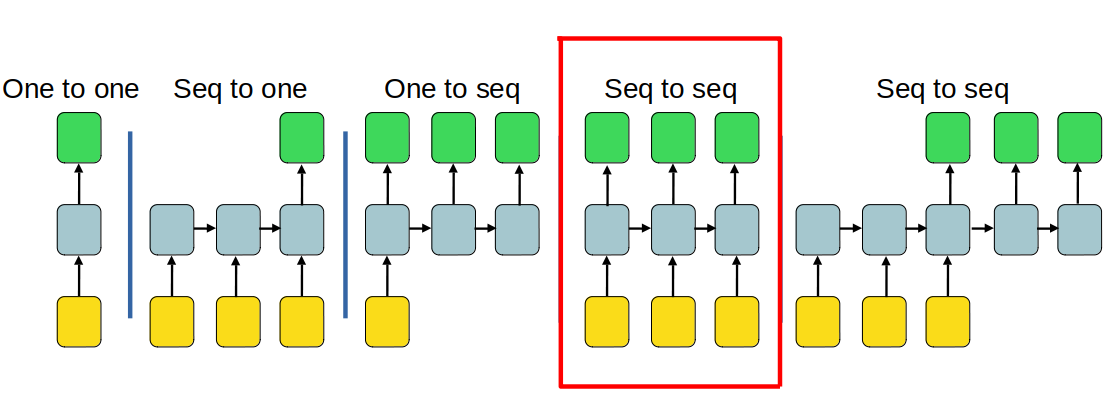
\includegraphics{figure/application_type1.png}}
  \end{figure}
\end{frame}

\begin{vbframe}{RNNs --- Language Modelling}
  \begin{itemize}
    \item We already built a \enquote{sequence-to-one} RNN model for sentiment analysis.
    \item Another common NLP task is \textbf{language modelling}.
    \item Input: word/character, one-hot encoded.
    \item Output: probability distribution over words/characters given previous words: $$\P(y^{[1]}, \dots, y^{[T]}) = \displaystyle \prod_{i=1}^{T} \P(y^{[i]}|y^{[1]}, \dots, y^{[i-1]})$$
    \item[] $\to$ given previous characters, the RNN models the probability distribution of the next character.
   \end{itemize}
\end{vbframe}

\begin{vbframe}{RNNs --- Language Modelling}
  \begin{itemize}
  \item We feed the characters in \enquote{hello} one at a time to a \enquote{seq-to-seq} RNN.
  \item \enquote{h}, \enquote{e}, \enquote{l}, \enquote{o} are one-hot coded as length-4 vectors (ignoring \texttt{<eos>}); the output layer has 4 neurons, one per character.
  \item At each time step, the RNN outputs a softmax probability distribution over the 4 possible next characters.
  \item If trained on English text:
    \begin{itemize}
      \item \enquote{e} should be likely given \enquote{h}.
      \item \enquote{l} should be likely given \enquote{he}.
      \item \enquote{l} should \textbf{also} be likely given \enquote{hel}.
      \item and \enquote{o} should be likely given \enquote{hell}.
    \end{itemize}
  \end{itemize}
\end{vbframe}

\frame{
\frametitle{RNNs --- Language Modelling}
  \begin{figure}
      \only<1>{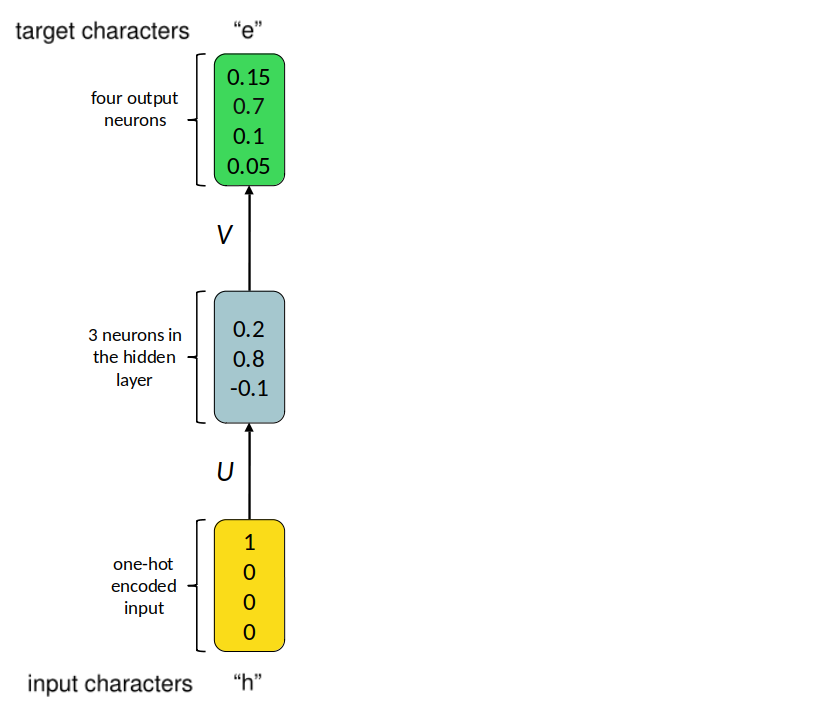
\includegraphics[width=6.5cm]{figure/m2many1.png}}%
      \only<2>{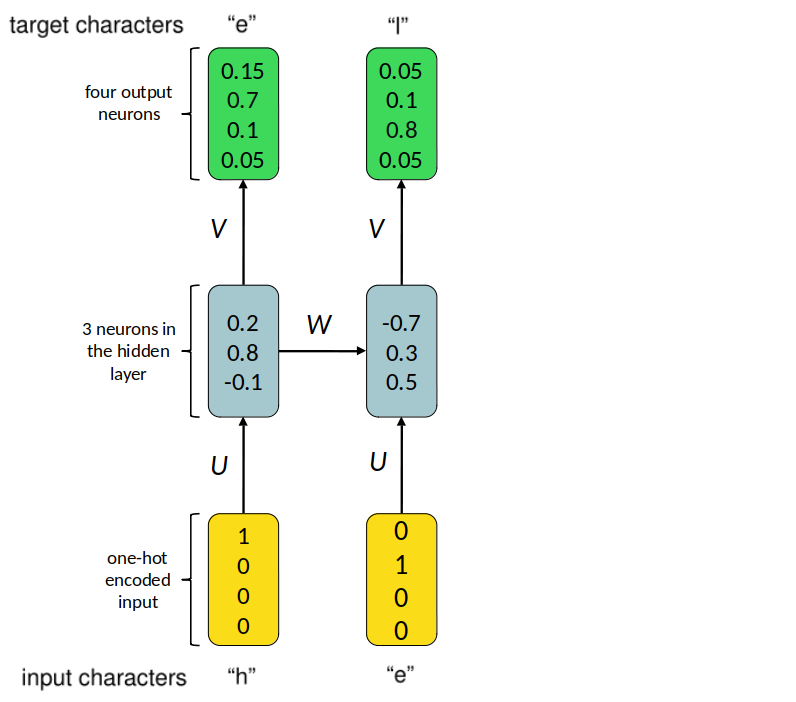
\includegraphics[width=6.5cm]{figure/m2many2.png}}%
      \only<3>{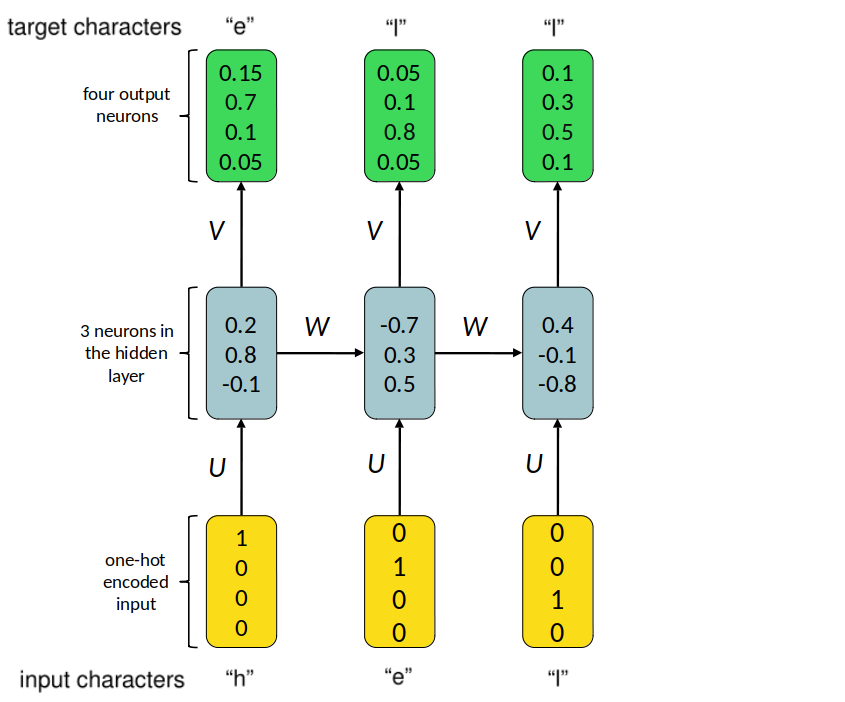
\includegraphics[width=6.5cm]{figure/m2many3.png}}%
      \only<4>{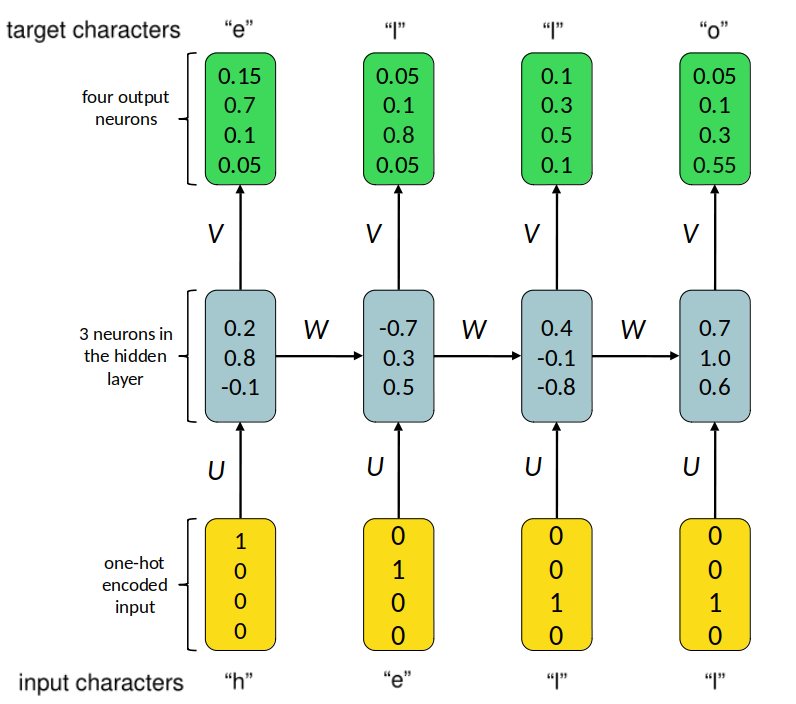
\includegraphics[width=6.5cm]{figure/m2many4.png}}%
      \only<5>{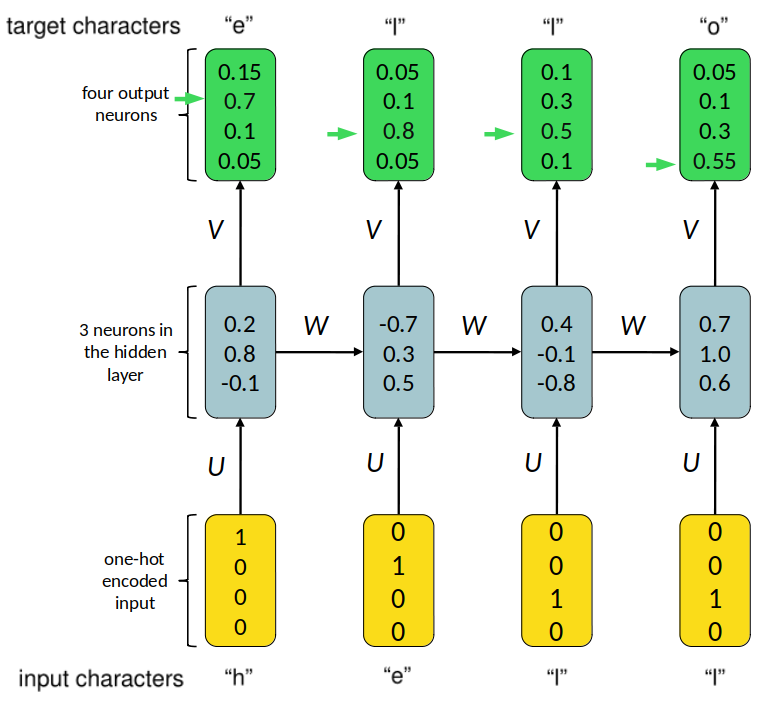
\includegraphics[width=6.5cm]{figure/m2many5.png}}%
  \end{figure}
  \begin{itemize}
    \only<1>{\item[] The probability of \enquote{e} should be high, given the context of \enquote{h}.}
    \only<2>{\item[] The probability of \enquote{l} should be high, given the context of \enquote{he}.}
    \only<3>{\item[] The probability of \enquote{l} should \textbf{also} be high, given the context of \enquote{hel}.}
    \only<4>{\item[] The probability of \enquote{o} should be high, given the context of \enquote{hell}.}
    \only<5>{\item[] During training, our goal is to increase confidence for the correct letters (green arrows) and decrease it for all others.}
  \end{itemize}
}

\begin{vbframe} {Word Embeddings}
\begin{figure}
\vspace{-0.5cm}
      \centering
      \scalebox{0.65}{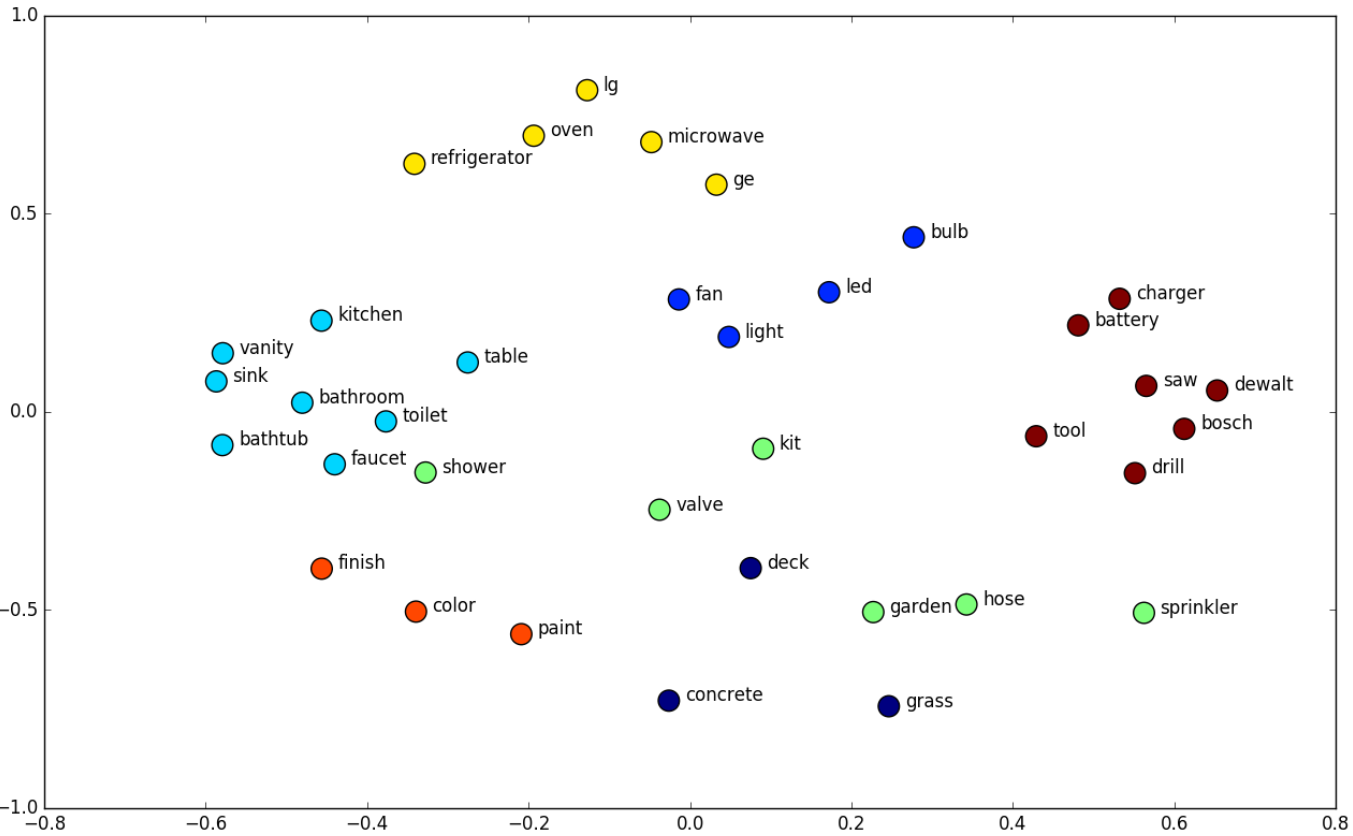
\includegraphics{figure/embed1.png}}
      \caption{Two-dimensional embedding space. The embedding space is typically much higher-dimensional (Ruizendaal, 2018).}
      \vspace{-0.7cm}
        \end{figure}
  \begin{itemize}
    \item Instead of one-hot representations, it is standard practice to encode each word as a dense (not sparse) vector of fixed size, capturing its underlying semantic content.
    \item Similar words are embedded close to each other in a lower-dimensional embedding space.
                \framebreak
    \item The embedding dimensionality is typically \text{much} smaller than the dictionary size.
    \item Using them gives a \enquote{warm start} for any NLP task --- an easy way to incorporate prior knowledge, and a rudimentary form of \textbf{transfer learning}.
    \item Two popular approaches to learn word embeddings: \textbf{word2vec} (Google) and \textbf{GloVe} (Stanford). Typically 100 to 1000 dimensional.
    \item These embeddings capture meaning to an extent, but not the \textit{context}-dependent semantics of a word, since each word has one static precomputed representation --- e.g.\ \enquote{bank} could mean a financial institution or a river bank.
  \end{itemize}
\end{vbframe}

\begin{frame}
\vspace{15mm}
\hspace{25mm} \textbf{\LARGE{Seq-to-Seq (Type II)}}
\begin{figure}
      \centering
      \scalebox{0.9}{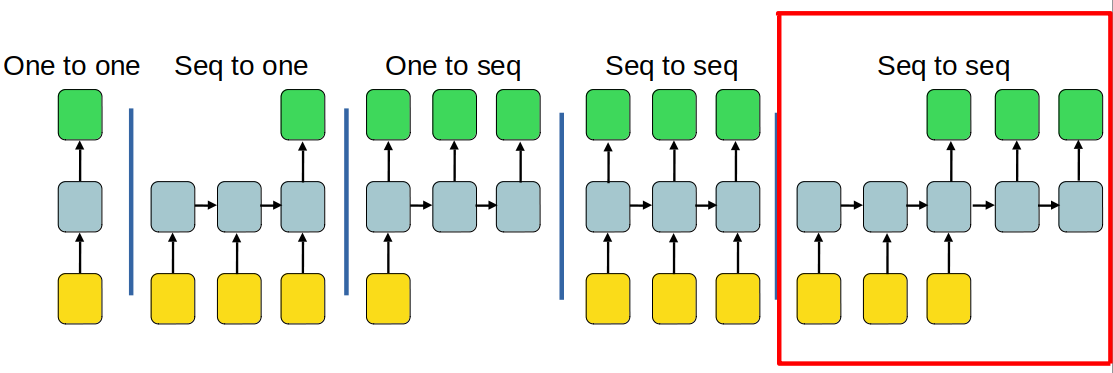
\includegraphics{figure/application_type2.png}}
  \end{figure}
\end{frame}

\begin{vbframe}{Encoder-Decoder Network}
  \begin{itemize}
    \item For applications such as question answering, dialogue systems, or machine translation, the network needs to map an input sequence to an output sequence of \textbf{different length}.
    \item This is what an encoder-decoder (a.k.a.\ sequence-to-sequence) architecture enables.
    \end{itemize}
 \framebreak
  \begin{figure}
    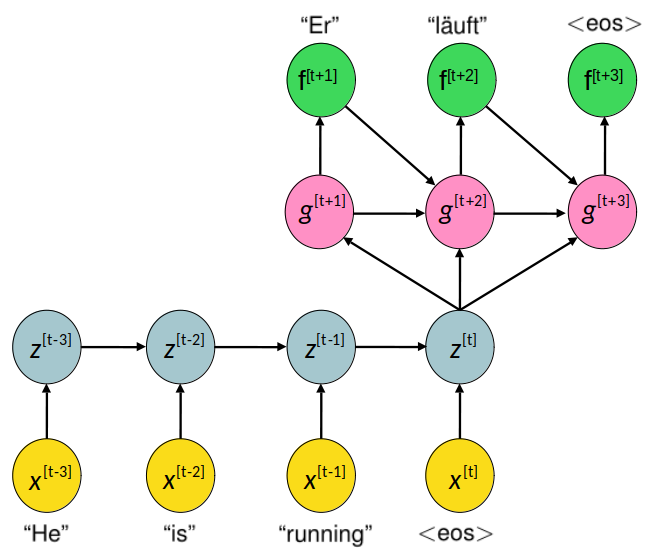
\includegraphics[width=7cm]{figure/seq2seq_2.png}
    \caption{Encoder-decoder allows an RNN to process different-length input and output sequences. Information from the input is encoded in the context vector (here, the final hidden state), passed to every decoder hidden state, which produces the target sequence.}
  \end{figure}
    \begin{itemize}
    \item An encoder RNN processes the input sequence (length $n_x$) and computes a fixed-length context vector $C$, usually the final hidden state or a simple function of the hidden states.
    \item One time step at a time, information from the input is added to the hidden state and passed forward through the encoder's recurrent connections.
    \item $C$ summarizes important information from the input --- e.g.\ the intent of a question, or the meaning of a text to translate.
    \item The decoder RNN uses this to predict the output sequence (length $n_y$, which may differ from $n_x$).
    \item In machine translation, the decoder is a language model with recurrent connections between the output at one time step and the hidden state at the next, as well as between hidden states:
    $$\P(y^{[1]}, \dots, y^{[n_y]}|\textbf{x}^{[1]},  \dots, \textbf{x}^{[n_x]}) = \displaystyle \prod_{t=1}^{n_y} p(y^{[t]}|C; y^{[1]}, \dots, y^{[t-1]})$$
    \item Trained jointly to minimize the translation error given a source sentence.
    \item Each conditional probability is $$p(y^{[t]}|y^{[1]}, \dots, y^{[t-1]};C) = f(y^{[t-1]}, g^{[t]}, C)$$ where $f$ is a non-linear function (e.g.\ tanh) and $g^{[t]}$ is the decoder's hidden state.
  \end{itemize}
\end{vbframe}
%%%%%%%%%%%%%%%%%%%%%%%%%%%%%%%%%%%%%%%%%%%%%%%%%%%%%%%%%%%%%%%%%%
%%%%%%%%%%%%%%%%%%          REFERENCES          %%%%%%%%%%%%%%%%%%
%%%%%%%%%%%%%%%%%%%%%%%%%%%%%%%%%%%%%%%%%%%%%%%%%%%%%%%%%%%%%%%%%%
\begin{vbframe}
\frametitle{References}
\footnotesize{
\begin{thebibliography}{99}
\bibitem[(Vinyals et al., 2014)]{rnn1} Vinyals, O., Toshev, A., Bengio, S., \& Erhan, D. (2014). \textit{Show and Tell: A Neural Image Caption Generator.}
\bibitem[(Ruizendaal, 2018)]{rnn2} Ruizendaal, R. (2018, October 21). \textit{Using deep learning for structured data with entity embeddings}. Medium. \url{https://towardsdatascience.com/deep-learning-structured-data-8d6a278f3088}
\bibitem[(Sutskever et al., 2014)]{rnn3} Sutskever, I., Vinyals, O., \& Le, Q. V. (2014). \textit{Sequence to Sequence Learning with Neural Networks.}
\end{thebibliography}
}
\end{vbframe}

%%%%%%%%%%%%%%%%%%%%%%%%%%%%%%%%%%%%%%%%%%%%%%%%%%%%%%%%%%%%%%%%%%
\section{Unsupervised Learning}
%%%%%%%%%%%%%%%%%%%%%%%%%%%%%%%%%%%%%%%%%%%%%%%%%%%%%%%%%%%%%%%%%%

\begin{vbframe}{Unsupervised Learning}
  \begin{itemize}
    \item So far, we have applied neural networks to \textbf{supervised learning}: labeled data $(\pmb{x}^{(1)}, \pmb{y}^{(1)}), \dots, (\pmb{x}^{(n)}, \pmb{y}^{(n)})$, exploited to learn a function mapping $\pmb{x}$ to $\pmb{y}$ (classification, regression, \ldots).
    \item In \textbf{unsupervised learning}, training data consists of unlabeled input points $\pmb{x}^{(1)}, \dots, \pmb{x}^{(n)}$, and the goal is to learn some underlying hidden structure of the data.
  \end{itemize}
\framebreak
Two motivating examples, both central to deep learning:
  \begin{itemize}
    \item[] \textbf{Feature extraction / representation learning}: features learned from unlabeled data improve performance in a supervised (or semi-supervised) setting. This is exactly what an \textbf{autoencoder} does --- covered next.
    \item[] \textbf{Density fitting / generative modeling}: learn $p_{\text{data}}$ itself, to generate new data, detect outliers, or reconstruct missing/corrupted inputs. This is what a \textbf{Variational Autoencoder} does --- covered later in this session.
  \end{itemize}
\end{vbframe}

%%%%%%%%%%%%%%%%%%%%%%%%%%%%%%%%%%%%%%%%%%%%%%%%%%%%%%%%%%%%%%%%%%
\section{Autoencoders: Basic Principle}
%%%%%%%%%%%%%%%%%%%%%%%%%%%%%%%%%%%%%%%%%%%%%%%%%%%%%%%%%%%%%%%%%%

\begin{vbframe}{Autoencoder --- Task and Structure}
  \begin{itemize}
  \item Autoencoders (AEs) are NNs for unsupervised learning of a good, lower-dimensional \textbf{representation} $\mathbf{z}$ (the \textbf{code}) from unlabeled training data.
  \item An AE consists of two parts:
  \begin{itemize}
            \item \textbf{encoder}: maps $\xv$ to the low-dimensional latent variable $\mathbf{z} = enc(\xv)$.
            \item \textbf{decoder}: maps $\mathbf{z}$ back to a reconstruction $\hat {\mathbf{x}} = dec(\mathbf{z})$ of $\xv$.
  \end{itemize}
    \item The loss uses no labels, measuring reconstruction quality against the input: $$L\left(\xv, dec(enc(\xv))\right)$$
  \end{itemize}
\framebreak
  The general structure of an AE as a computational graph:
  \begin{figure}
    \centering
    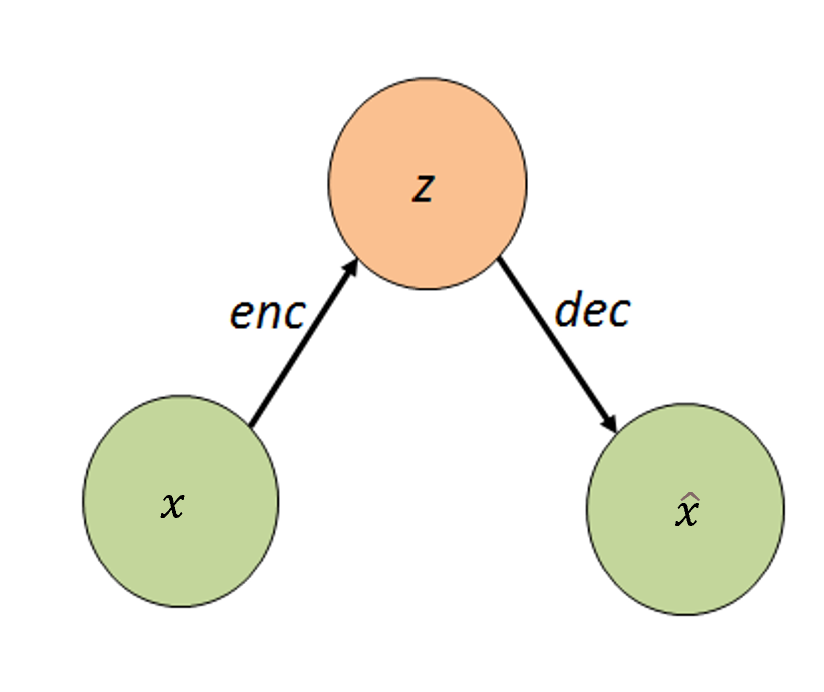
\includegraphics[width=4.5cm]{figure/autoencoders_basic_structure_updated.png}
  \end{figure}
\end{vbframe}

\begin{frame}{Undercomplete Autoencoders}
  \only<1>{
    \begin{itemize}
      \item A naive AE would simply learn the identity $dec(enc(\xv)) = \mathbf{\hat x}$ --- not useful.
    \end{itemize}
    \begin{figure}
    \centering
    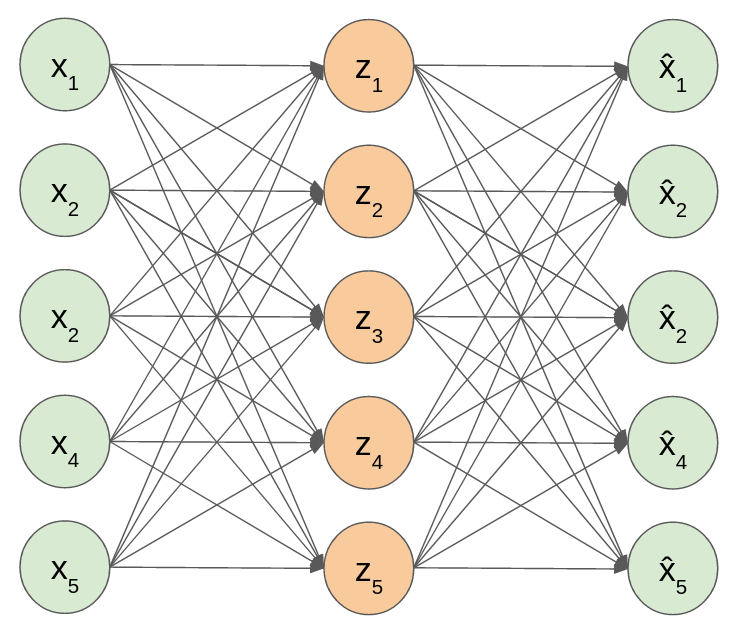
\includegraphics[width=0.55\textwidth]{figure/AE_naive1.png}
    \end{figure}
  }
  \only<2>{
    \begin{itemize}
      \item Therefore we introduce a \enquote{bottleneck} layer: restrict the architecture such that $\text{dim}(\mathbf{z}) < \text{dim}(\xv)$ --- such an AE is called \textbf{undercomplete}.
      \item[$\rightarrow$] With fewer hidden neurons than input neurons, it is forced to capture only the most salient features, learning a \enquote{compressed} representation of the input.
    \end{itemize}
    \begin{figure}
    \centering
    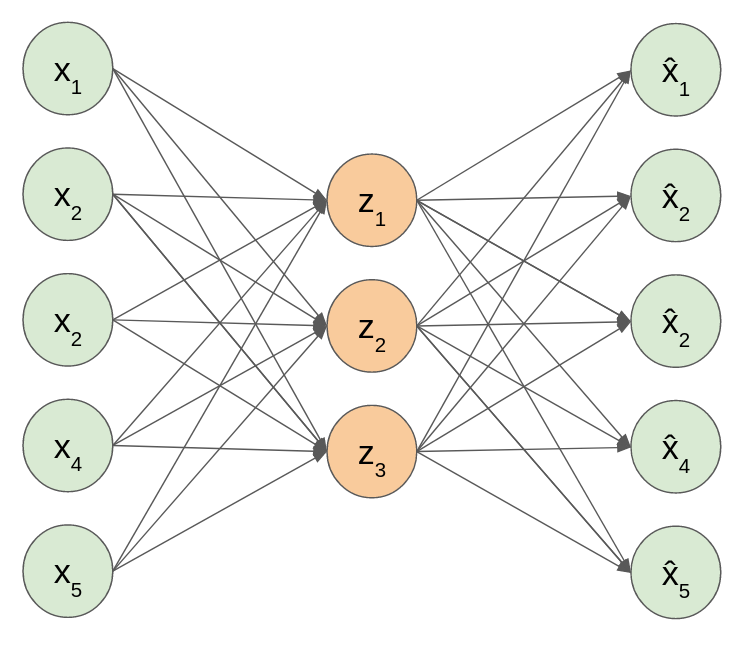
\includegraphics[width=0.42\textwidth]{figure/AE_undercomplete.png}
    \end{figure}
  }
\end{frame}

\frame{
\frametitle{Experiment: Learn to Encode MNIST}
  \begin{itemize}
    \item Compress MNIST: train undercomplete AEs with different dimensions of the internal representation $\mathbf{z}$ (different \enquote{bottleneck} sizes).
  \end{itemize}
  \center
  \begin{figure}
    \only<1>{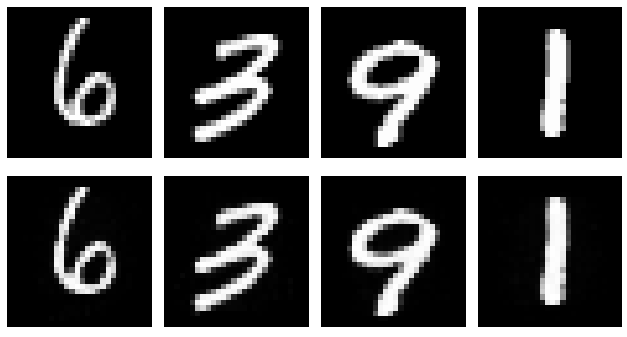
\includegraphics[width=6.5cm]{figure/784.png}}%
    \only<2>{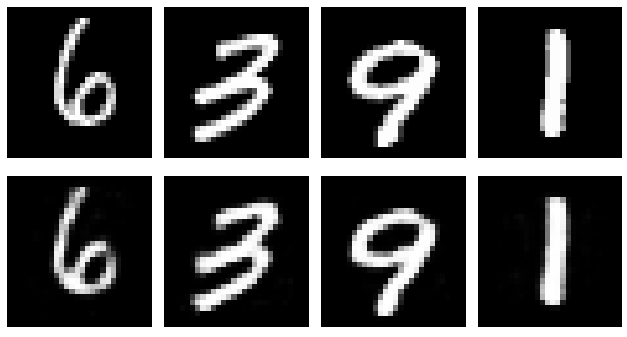
\includegraphics[width=6.5cm]{figure/64.png}}%
    \only<3>{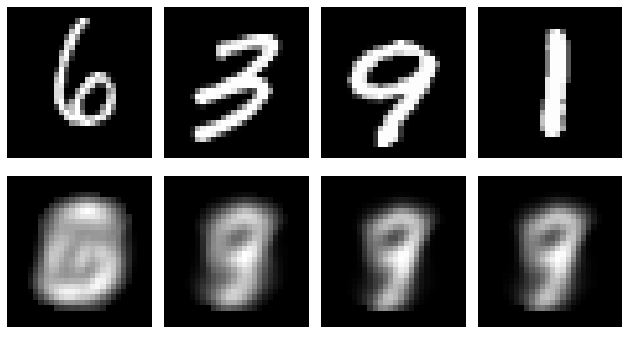
\includegraphics[width=6.5cm]{figure/1.png}}%
    \caption{\footnotesize Top row: original digits; bottom row: reconstructions.}
  \end{figure}
  \begin{itemize}
    \only<1>{\item $dim(\mathbf{z}) = 784 = dim(\xv)$.}
    \only<2>{\item $dim(\mathbf{z}) = 64$.}
    \only<3>{\item $dim(\mathbf{z}) = 1$.}
  \end{itemize}
}

\begin{vbframe}{AEs as Principal Component Analysis}
  \begin{itemize}
    \item Consider an undercomplete AE with a \textbf{linear} encoder and a \textbf{linear} decoder.
    \item Using the L2-loss $\|\xv-dec(enc(\xv))\|^2_2$ with inputs normalized to zero mean, we want the \textbf{linear projection} of the data with minimal L2-reconstruction error.
    \begin{figure}
      \centering
      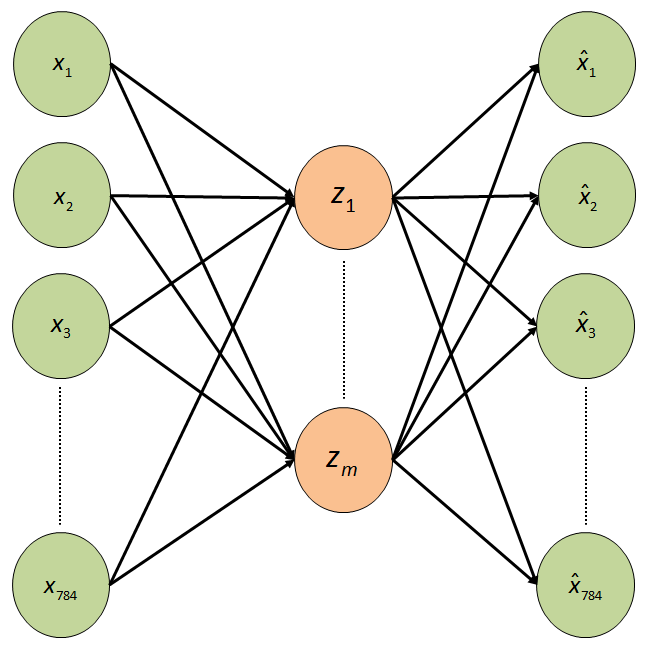
\includegraphics[width=0.3\textwidth]{figure/autoencoder_mnist_example.png}
    \end{figure}
    \framebreak
    \item It can be shown that the optimal solution is an \textbf{orthogonal} linear transformation (a rotation of the coordinate system), given by the $\text{dim}(\bm{z}) = k$ singular vectors with the largest singular values.
    \begin{figure}
    \centering
    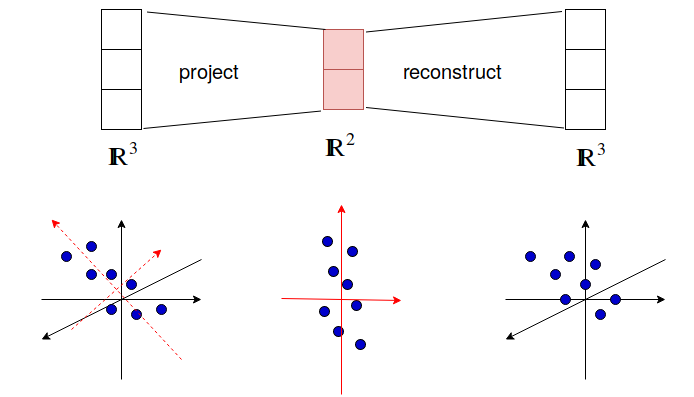
\includegraphics[width=0.7\textwidth]{figure/PCA_AE.png}
    \end{figure}
    \framebreak
    \item This is equivalent to \textbf{Principal Component Analysis (PCA)}: an orthogonal transformation converting correlated variables into linearly uncorrelated \textbf{principal components}, with the first component having the largest possible variance.
    \item The two formulations are equivalent: \enquote{Find a linear projection into a $k$-dimensional space that \ldots}
    \begin{itemize}
      \item \enquote{\ldots minimizes the L2-reconstruction error} (AE-based).
      \item \enquote{\ldots maximizes the variance of the projected datapoints} (statistical).
    \end{itemize}
    \item An AE with a non-linear decoder/encoder is a non-linear generalization of PCA.
    \begin{figure}
    \centering
    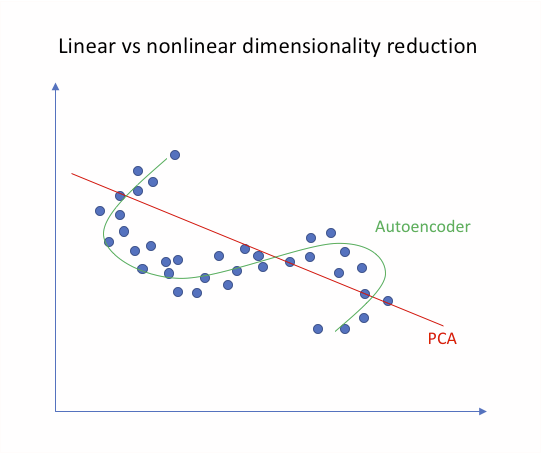
\includegraphics[width=0.3\textwidth]{figure/manifold1.png}
    \caption{AEs can learn nonlinear manifolds (Jordan, 2018).}
    \end{figure}
  \end{itemize}
\end{vbframe}

%%%%%%%%%%%%%%%%%%%%%%%%%%%%%%%%%%%%%%%%%%%%%%%%%%%%%%%%%%%%%%%%%%
\section{Regularized Autoencoders}
%%%%%%%%%%%%%%%%%%%%%%%%%%%%%%%%%%%%%%%%%%%%%%%%%%%%%%%%%%%%%%%%%%

\begin{vbframe}{Overcomplete AE --- Problem}
  Overcomplete AE (code dimension $\geq$ input dimension): even a linear AE can copy the input to the output without learning anything useful. How can an overcomplete AE be useful?
\begin{figure}[h]
    \centering
    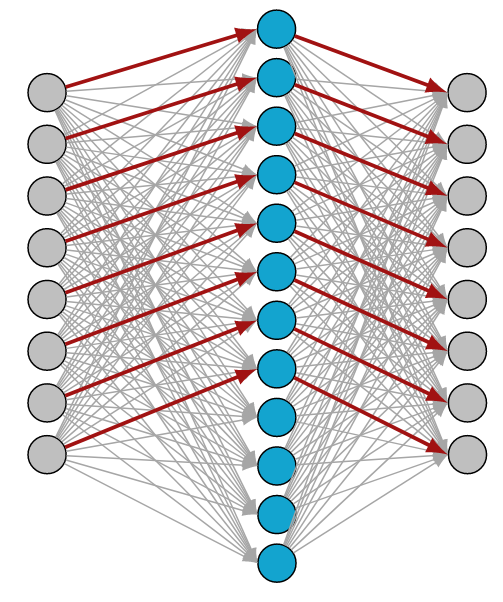
\includegraphics[width=0.3\linewidth]{figure/AE_overcomplete2.png}
    \caption{Overcomplete AE that learned to copy its input to the hidden layer, then to the output (Ponti et al., 2016).}
\end{figure}
    \begin{itemize}
       \item Goal: choose code dimension and encoder/decoder capacity based on the problem.
       \item \textbf{Regularized AEs} modify the loss function to prevent trivially copying the input, and to encourage additional properties.
        \item Examples:
            \begin{itemize}
                \item \textbf{Sparse AE:} sparsity of the representation.
                \item \textbf{Denoising AE}: robustness to noise.
            \end{itemize}
    \end{itemize}
    $\Rightarrow$ A regularized AE can be overcomplete and nonlinear, but still learn something useful about the data distribution.
\end{vbframe}

\begin{vbframe}{Sparse Autoencoder}
\begin{itemize}
  \item \textbf{Idea:} regularize with a sparsity constraint: $$L(\xv, dec(enc(\xv))) + \lambda \|\bm{z}\|_1$$
\item Keeps the number of active neurons per training input low, forcing the model to respond to unique statistical features of the input.
\item \textbf{Application:} beyond classic feature learning for downstream tasks, sparse AEs are now used to decompose the internal activations of trained neural networks (e.g.\ LLMs) into human-interpretable, non-overlapping features --- a key tool in mechanistic interpretability research (Anthropic, 2024).
\end{itemize}
\begin{figure}[h]
    \centering
    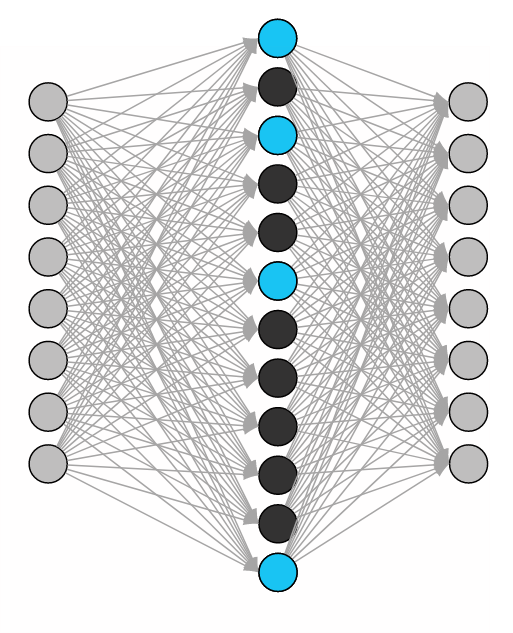
\includegraphics[width=0.25\linewidth]{figure/AE_sparse.png}
    \caption{Sparse Autoencoder (Ponti et al., 2016).}
\end{figure}
\end{vbframe}

\begin{vbframe}{Denoising Autoencoders (DAE)}
The denoising autoencoder (DAE) receives a corrupted data point as input and is trained to predict the original, uncorrupted data point.
    \begin{itemize}
       \item Idea: the representation should be robust to noise.
       \item Produce a corrupted version $\tilde{\xv}$ of $\xv$, e.g.\ by
     \begin{itemize}
        \item random assignment of a subset of inputs to 0,
      \item adding Gaussian noise.
       \end{itemize}
        \item Modified reconstruction loss: $L(\xv, \color{red}{dec(enc(\tilde{\xv}))}\color{black}{)}$ $\rightarrow$ denoising AEs must learn to undo this corruption.
    \end{itemize}
\framebreak
  \begin{figure}
    \centering
    \scalebox{0.42}{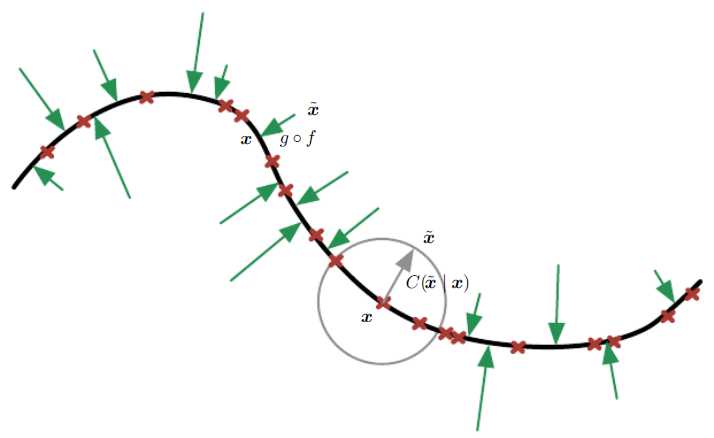
\includegraphics{figure/denoising_autoencoder.png}}
    \caption{Denoising autoencoders --- \enquote{manifold perspective} (Goodfellow et al., 2016).}
  \end{figure}
  \begin{itemize}
    \item A DAE is trained to map a corrupted point $\tilde{\xv}$ back to the original $\xv$: the vector $dec(enc(\tilde{\xv})) - \tilde{\xv}$ points approximately towards the nearest point on the data manifold.
    \item Thus, the DAE learns a vector field pointing back onto the manifold, indicated by the green arrows.
  \end{itemize}
\end{vbframe}

\begin{frame}{Experiment: Encode MNIST with a DAE}
  \begin{itemize}
    \item We corrupt the MNIST data with Gaussian noise and then try to denoise it as well as possible.
    \item To corrupt the input, we randomly add or subtract uniformly-distributed values to each image entry.
  \end{itemize}
  \begin{figure}
    \centering
    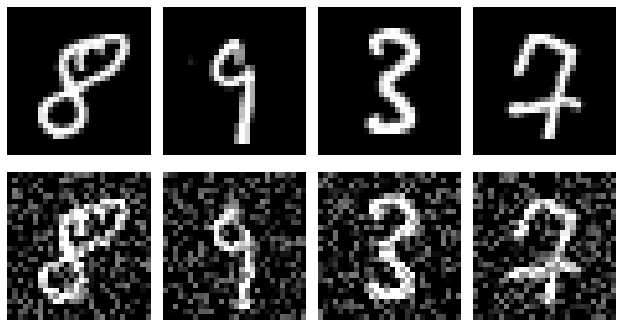
\includegraphics[width=7cm]{figure/mnist_noise.png}
    \caption{Top row: original data; bottom row: corrupted MNIST data.}
  \end{figure}
\end{frame}

\frame{
\frametitle{Experiment: Encode MNIST with a DAE}
  \center
  \begin{figure}
    \only<1>{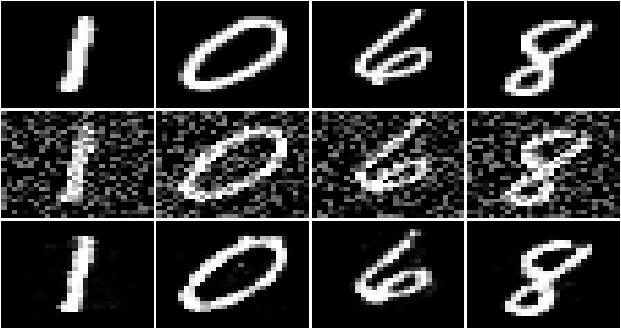
\includegraphics[width=6.5cm]{figure/denoised_1568_2.png}}%
    \only<2>{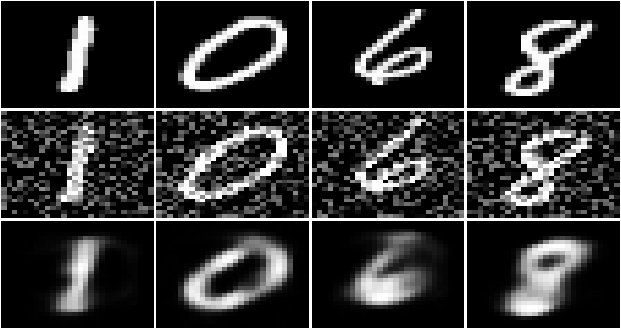
\includegraphics[width=6.5cm]{figure/denoised_8_2.png}}%
    \caption{\footnotesize Top row: original digits; middle: corrupted; bottom: denoised/reconstructed (prediction).}
  \end{figure}
  \vspace{-0.1cm}
  \begin{itemize}
 \only<1>{\item $dim(\pmb{z}) = 1568$ (overcomplete).}
    \only<2>{\item $dim(\pmb{z}) = 8$.}
  \end{itemize}
}

%%%%%%%%%%%%%%%%%%%%%%%%%%%%%%%%%%%%%%%%%%%%%%%%%%%%%%%%%%%%%%%%%%
%%%%%%%%%%%%%%%%%%%%%%%%%%%%%%%%%%%%%%%%%%%%%%%%%%%%%%%%%%%%%%%%%%
%%%%%%%%%%%%%%%%%%          REFERENCES          %%%%%%%%%%%%%%%%%%
%%%%%%%%%%%%%%%%%%%%%%%%%%%%%%%%%%%%%%%%%%%%%%%%%%%%%%%%%%%%%%%%%%
\begin{vbframe}
\frametitle{References}
\footnotesize{
\begin{thebibliography}{99}
\bibitem[(Goodfellow et al., 2016)]{ae7} Goodfellow, I., Bengio, Y., \& Courville, A. (2016). \textit{Deep Learning}. MIT Press.
\bibitem[(Jordan, 2018)]{ae9} Jordan, J. (2018, March 19). \textit{Introduction to autoencoders}. \url{https://www.jeremyjordan.me/autoencoders/}
\bibitem[(Ponti et al., 2016)]{ae10} Ponti, M. A., Ribeiro, L. S. F., Nazare, T. S., Bui, T., \& Collomosse, J. (2017). Everything You Wanted to Know about Deep Learning for Computer Vision but Were Afraid to Ask. \textit{2017 30th SIBGRAPI Conference on Graphics, Patterns and Images Tutorials}, 17--41.
\bibitem[(Anthropic, 2024)]{ae13} Anthropic. (2024). \textit{Scaling Monosemanticity: Extracting Interpretable Features from Claude 3 Sonnet}. Transformer Circuits Thread. \url{https://transformer-circuits.pub/2024/scaling-monosemanticity/}
\end{thebibliography}
}
\end{vbframe}

%%%%%%%%%%%%%%%%%%%%%%%%%%%%%%%%%%%%%%%%%%%%%%%%%%%%%%%%%%%%%%%%%%
\section{Variational Autoencoders (VAE)}
%%%%%%%%%%%%%%%%%%%%%%%%%%%%%%%%%%%%%%%%%%%%%%%%%%%%%%%%%%%%%%%%%%

\begin{frame}
\frametitle{Variational Autoencoder (VAE): Intuition}
Independently proposed by:
\small{
\begin{itemize}
\item Kingma and Welling, \emph{Auto-Encoding Variational Bayes}, ICLR 2014
\item Rezende, Mohamed and Wierstra, \emph{Stochastic back-propagation and variational inference in deep latent Gaussian models.} ICML 2014
\end{itemize}}
\vspace{1mm}
Conventional AEs compute a deterministic feature vector describing the input's attributes in latent space:
                \begin{figure}
                \centering
                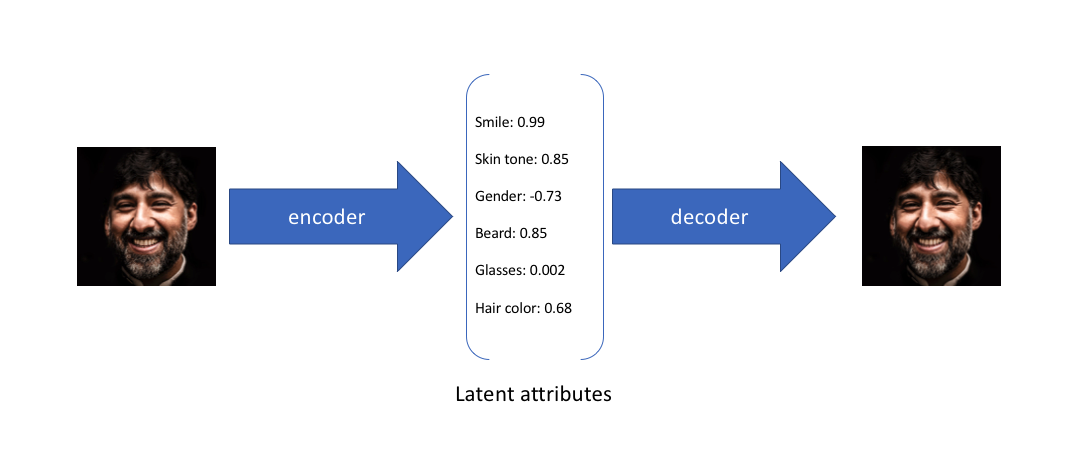
\includegraphics[width=3.8cm]{figure/ae_intution.png}
                \vspace{-8pt}
                \caption{\tiny{Source: Jordan (2018)}}
                \end{figure}
\begin{itemize}
\item The key difference in VAEs: they use a \textbf{variational} approach to learn the latent representation, allowing observations in latent space to be described \textbf{probabilistically}.
\end{itemize}
\end{frame}

\begin{frame}
\frametitle{Variational Autoencoder (VAE): Intuition}
                \begin{figure}
                \centering
                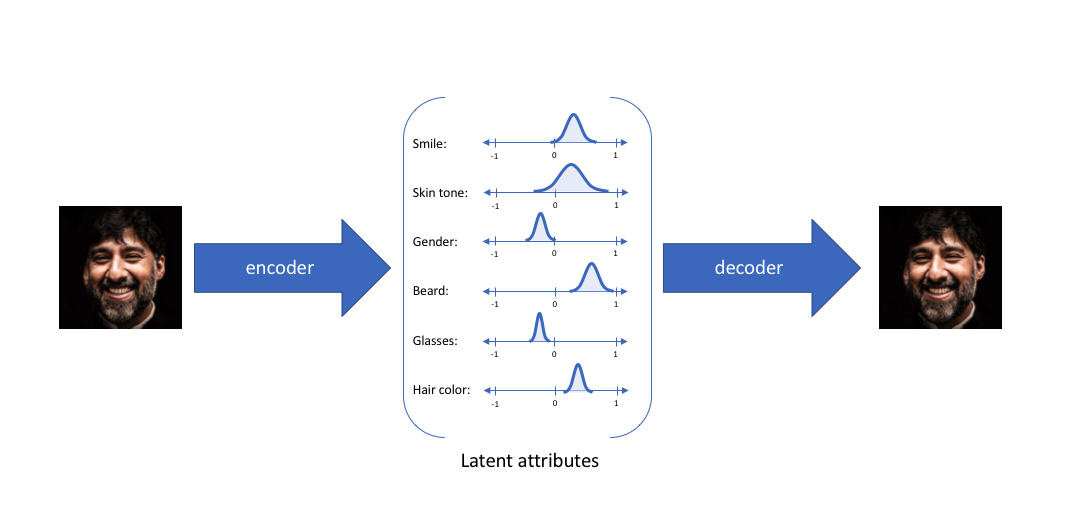
\includegraphics[width=7cm]{figure/vae_intution.png}
                \vspace{-8pt}
                \caption{\tiny{Source: Jordan (2018)}}
                \end{figure}
\begin{itemize}
\item Describe each latent attribute as a probability distribution.
\item This allows modelling uncertainty in the input data.
\end{itemize}
\end{frame}

\begin{frame}
\frametitle{VAE: Statistical Motivation}
\begin{itemize}
\item Suppose a hidden variable $z$ generates an observation $x$.
\item By training the VAE, we want to determine the distribution of $z$ and compute $p(z|x)$: $$p\left( {z|x} \right) = \frac{{p\left( {x|z} \right)p\left( z \right)}}{{p\left( x \right)}}$$
\item Computing $p(x)$ is difficult, since it is an intractable integral: $$p\left( x \right) = \int {p\left( {x|z} \right)p\left( z \right)dz}$$
\item Instead, we apply \textbf{variational inference}: approximate $p(z|x)$ by a tractable distribution $q(z|x)$ that is very similar to it.
\end{itemize}
\end{frame}

\begin{frame}
\frametitle{VAE: Statistical Motivation}
\begin{itemize}
\item KL divergence measures the difference between two distributions. To make $q(z|x)$ similar to $p(z|x)$, we could minimize $$\min KL\left( {q\left( {z|x} \right)||p\left( {z|x} \right)} \right)$$
\item This is equivalent to maximizing: $$\max {E_{q\left( {z|x} \right)}}\log p\left( {x|z} \right) - KL\left( {q\left( {z|x} \right)||p\left( z \right)} \right)$$
\item The first term is the reconstruction likelihood; the second ensures the learned $q$ stays close to the true prior $p(z)$.
\end{itemize}
\end{frame}

\begin{frame}
\frametitle{VAE: Statistical Motivation}
\begin{itemize}
\item $p(z)$ is often assumed Gaussian $\rightarrow$ determining $q(z|x)$ reduces to estimating $\mu$ and $\sigma$.
\item We use a neural network to estimate $q(z|x)$ (the encoder) and the decoder network to model $p(x|z)$.
\end{itemize}
                \begin{figure}
                \centering
                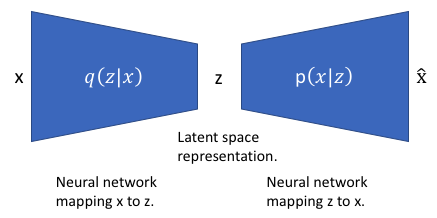
\includegraphics[width=9cm]{figure/vae.png}
                \vspace{-6pt}
                \caption{\tiny{Source: Jordan (2018)}}
                \end{figure}
\end{frame}

\begin{frame}
\frametitle{VAE Training}
                \begin{figure}
                \centering
                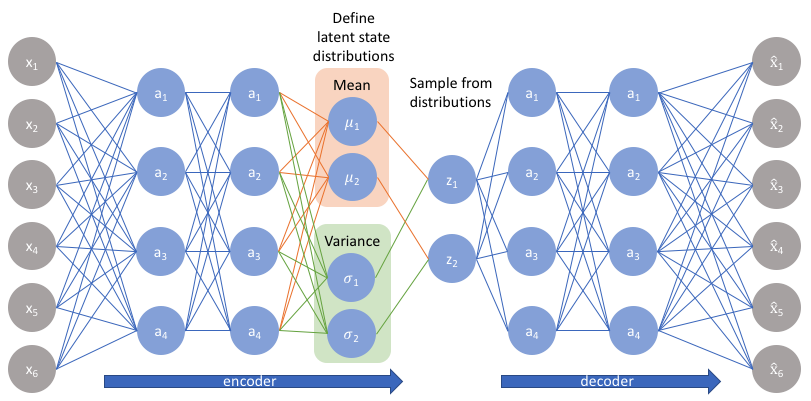
\includegraphics[width=3.5cm]{figure/vae_training.png}
                \vspace{-6pt}
                \caption{\tiny{Source: Jordan (2018)}}
                \end{figure}
\begin{itemize}
\item Loss function (the \textbf{Evidence Lower BOund}, or \textbf{ELBO}): $$ L(\theta, \phi; x, z) = \underbrace{E_{q_{\phi} ({z|x})} \log p_{\theta} ({x|z})}_{\text{reconstruction term}} - \underbrace{KL ({q_{\phi} ({z|x})|| p_{\theta} (z)})}_{\text{stay-close-to-prior term}}$$
\item Maximizing the ELBO jointly maximizes reconstruction quality and keeps the encoder's distribution close to the prior.
\item Problem: the network contains a \textbf{sampling} step $\rightarrow$ we cannot backpropagate through it!
\end{itemize}
\end{frame}

\begin{frame}
\frametitle{Reparameterization Trick}
\begin{itemize}
\item We cannot backpropagate through random sampling --- what now?
\item Idea: \enquote{push} the random sampling out of the backpropagation path by \textbf{reparameterizing} it.
\item Instead of sampling $\mathbf{z}$ directly from $\mathcal{N}(\bm\mu_{\mathbf z}(\xv), \bm\sigma^2_{\mathbf z}(\xv))$, we sample a fixed noise source $\bm\epsilon \sim \mathcal{N}(\mathbf{0}, \mathbf{1})$ and compute $$\mathbf{z} = \bm\mu_{\mathbf z}(\xv) + \bm\sigma_{\mathbf z}(\xv) \odot \bm\epsilon$$
\item Now the only randomness is in $\bm\epsilon$, which does not depend on the network's parameters --- so gradients can flow through $\bm\mu_{\mathbf z}(\xv)$ and $\bm\sigma_{\mathbf z}(\xv)$ as usual.
\end{itemize}
                \begin{figure}
                \centering
                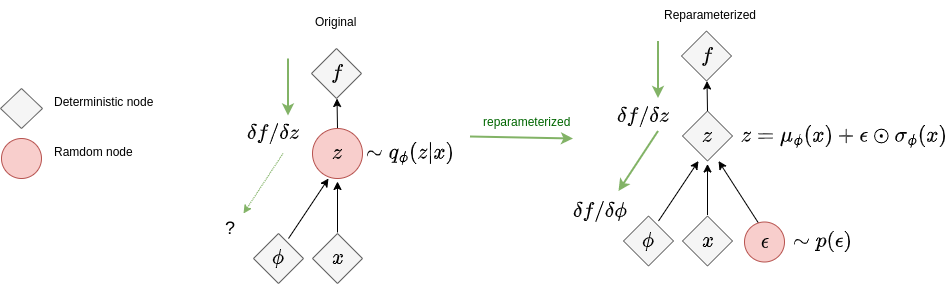
\includegraphics[width=7cm]{figure/vae_reparam.png}
                \end{figure}
\end{frame}

\frame{
    \frametitle{Variational Autoencoders as a Generative Model}
    \begin{itemize}
    \item New data can be generated by sampling from distributions in the latent space, then reconstructing via the decoder.
    \item A diagonal prior enforces independent latent variables $\rightarrow$ can encode different factors of variation.
    \end{itemize}
    \begin{figure}
    \centering
    \scalebox{0.22}{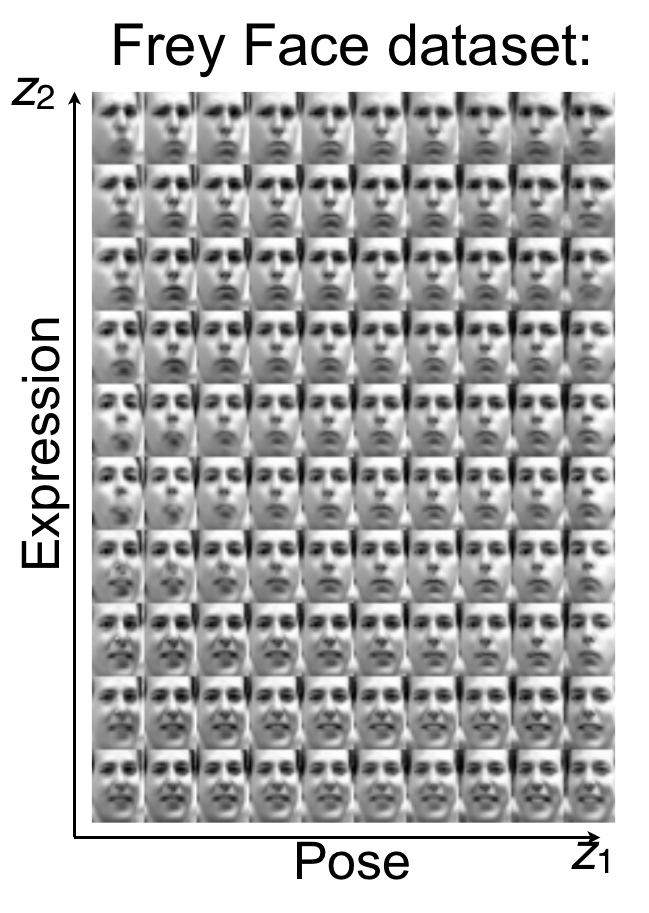
\includegraphics{figure/LatentVariables-FF.png}}
    \caption{\footnotesize Images generated by a VAE, superimposed on the latent vectors that generated them: dimension 1 encodes face position, dimension 2 encodes expression (Goodfellow et al., 2016).}
    \end{figure}
}

\frame{
    \frametitle{Samples from a Vanilla VAE}
    \begin{figure}
      \centering
      \scalebox{0.9}{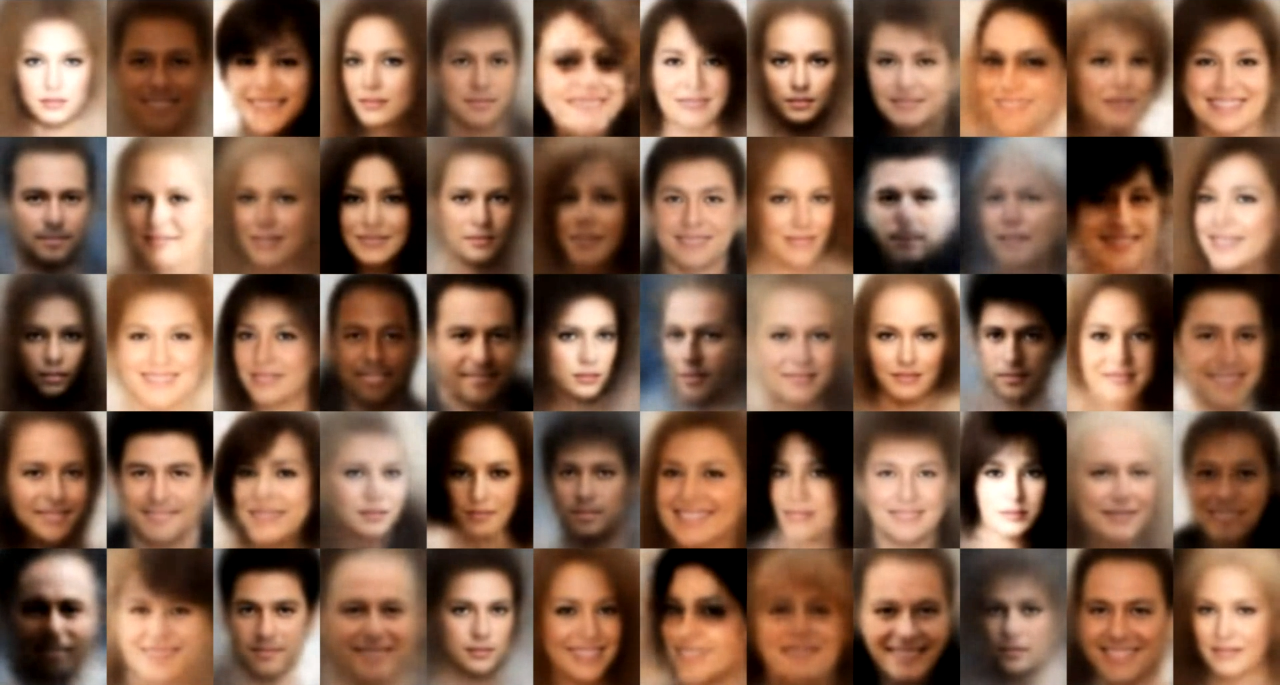
\includegraphics{figure/vae_faces.png}}
      \caption{\footnotesize Samples generated by a VAE trained on images of faces.}
    \end{figure}
}

\begin{frame}
\frametitle{Variational Autoencoders: Summary}
\begin{itemize}
  \item Probabilistic model $\rightarrow$ allows generating data.
  \item Intractable density $\rightarrow$ optimizes the variational lower bound (ELBO) instead.
  \item Trained by backpropagation, using the reparameterization trick.
  \item Pros:
    \begin{itemize}
      \item principled approach to generative models,
      \item the latent-space reparameterization is useful for other tasks too.
    \end{itemize}
  \item Cons:
    \begin{itemize}
      \item only maximizes a \textit{lower bound} of the likelihood,
      \item samples in standard VAEs are often blurrier than samples from other modern generative approaches.
    \end{itemize}
  \item Active area of research!
\end{itemize}
\end{frame}
%%%%%%%%%%%%%%%%%%%%%%%%%%%%%%%%%%%%%%%%%%%%%%%%%%%%%%%%%%%%%%%%%%
%%%%%%%%%%%%%%%%%%          REFERENCES          %%%%%%%%%%%%%%%%%%
%%%%%%%%%%%%%%%%%%%%%%%%%%%%%%%%%%%%%%%%%%%%%%%%%%%%%%%%%%%%%%%%%%
\begin{vbframe}
\frametitle{References}
\footnotesize{
\begin{thebibliography}{99}
\bibitem[(Jordan, 2018)]{vae1} Jordan, J. (2018). \textit{Variational Autoencoders}. \url{https://www.jeremyjordan.me/variational-autoencoders/}
\bibitem[(Goodfellow et al., 2016)]{vae2} Goodfellow, I., Bengio, Y., \& Courville, A. (2016). \textit{Deep Learning}. MIT Press.
\end{thebibliography}
}
\end{vbframe}

%%%%%%%%%%%%%%%%%%%%%%%%%%%%%%%%%%%%%%%%%%%%%%%%%%%%%%%%%%%%%%%%%%
\section{Transformer Outlook}
%%%%%%%%%%%%%%%%%%%%%%%%%%%%%%%%%%%%%%%%%%%%%%%%%%%%%%%%%%%%%%%%%%

\begin{vbframe}{Where This Is Going: Attention and Transformers}
  \begin{itemize}
    \item The encoder-decoder RNN squeezes an entire input sequence into a \textbf{single} fixed-length context vector $C$ --- Bahdanau et al. (2015) identify this as a bottleneck: the network must compress all information about a source sentence, regardless of its length, into one vector.
    \item Empirically, this bottleneck bites hard on long sentences: on the WMT'14 English-to-French task, a plain encoder-decoder's BLEU score collapses as sentence length grows past $\sim$20 words, while an attention-based model's stays essentially flat even past 50 words (Bahdanau et al., 2015).
    \item \textbf{Attention} fixes this by letting the decoder look back at \textit{all} encoder hidden states at every decoding step, learning which parts of the input matter most for the current output --- rather than compressing everything into one vector up front.
    \item This turns out to be a more fundamental idea than just an RNN add-on: Vaswani et al. (2017) show an architecture ``based solely on attention mechanisms, dispensing with recurrence and convolutions entirely'' --- and it set a new state of the art (28.4 BLEU on WMT'14 English-German, +2 BLEU over the best prior ensemble; 41.8 BLEU on English-French) while training in a fraction of the time of prior models.
    \item That architecture is the \textbf{Transformer} --- the subject of Session 7, in depth.
  \end{itemize}
\end{vbframe}

\begin{vbframe}{Why This Matters for Generative Models Too}
  \begin{itemize}
    \item Every generative model family in this session --- autoencoders, VAEs --- is defined by \textit{what} is being learned (a compressed code, a latent distribution), independent of \textit{which} network computes it.
    \item Any of them can use an RNN, a CNN, or a Transformer as their encoder/decoder --- the architectures in this session and CNNs (Session 5) are building blocks, not fixed pairings.
    \item In practice, Transformer-based encoders and decoders have now displaced RNNs in most large-scale sequence and generative models.
  \end{itemize}
\end{vbframe}

%%%%%%%%%%%%%%%%%%          REFERENCES          %%%%%%%%%%%%%%%%%%
\begin{vbframe}
\frametitle{References}
\footnotesize{
\begin{thebibliography}{99}
\bibitem[(Bahdanau et al., 2015)]{trans1} Bahdanau, D., Cho, K., \& Bengio, Y. (2015). \textit{Neural Machine Translation by Jointly Learning to Align and Translate}. Published as a conference paper at ICLR 2015. \url{https://arxiv.org/abs/1409.0473}
\bibitem[(Vaswani et al., 2017)]{trans2} Vaswani, A., Shazeer, N., Parmar, N., Uszkoreit, J., Jones, L., Gomez, A. N., Kaiser, {\L}., \& Polosukhin, I. (2017). \textit{Attention Is All You Need}. \url{https://arxiv.org/abs/1706.03762}
\end{thebibliography}
}
\end{vbframe}

%%%%%%%%%%%%%%%%%%%%%%%%%%%%%%%%%%%%%%%%%%%%%%%%%%%%%%%%%%%%%%%%%%
\section{License \& Attribution}
%%%%%%%%%%%%%%%%%%%%%%%%%%%%%%%%%%%%%%%%%%%%%%%%%%%%%%%%%%%%%%%%%%

\begin{vbframe}{License \& Attribution}
\begin{itemize}
\item RNN sections (Motivation and Mechanics; Worked Example and Use Cases; Computational Graph and Bidirectional RNNs; Backpropagation Through Time; LSTM and GRU; RNN Applications), Unsupervised Learning, Autoencoders (Basic Principle; Regularized Autoencoders), and Variational Autoencoders
adapted from \textbf{Introduction to Deep Learning (I2DL)}, Prof.\ Dr.\
Bernd Bischl, SLDS, LMU Munich. \url{https://github.com/slds-lmu/lecture_i2dl}
--- licensed \textbf{CC BY 4.0}: \url{https://creativecommons.org/licenses/by/4.0/}
\item The \enquote{Multi-Layer (Stacked) RNNs} frame is adapted from \textbf{Deep Learning for NLP (DL4NLP)}, SLDS, LMU Munich --- also licensed \textbf{CC BY 4.0}. This topic is not covered in I2DL's own RNN material; its diagram was redrawn independently rather than reusing the original's custom TikZ macros.
\item The \enquote{Transformer Outlook} bridge is original text written for this course, not adapted from I2DL, DL4NLP, or any other source.
\item Content in this deck has been merged, reordered, and (for VAE derivations) condensed from the originals; not used verbatim.
\end{itemize}
\end{vbframe}

\endlecture
\end{document}

